\graphicspath{{chapter2/}{manuscript/}}

\chapter{\textbf{}}

\begin{center}
\textbf{Sensitivity of tree species performance to climate and
competition changes across their range distribution} \\
Willian~Vieira, Andrew~MacDonald, Dominique~Gravel
\end{center}

\hypertarget{supplementary-material-1}{%
\section{Supplementary Material 1}\label{supplementary-material-1}}

\hypertarget{sec-model-fit}{%
\subsection{Model fit}\label{sec-model-fit}}

We assessed the growth, survival, and recruitment rates by examining
transitions between two measurements. While we fitted the growth and
survival functions at the individual level, recruitment was evaluated at
the plot level. Due to differences in measurement thresholds between the
FIA and Quebec protocols, we only considered individuals with a dbh
\(\ge\) 127 mm. Therefore, we quantified the ingrowth rate as the number
of individuals crossing the 127 mm threshold. We included trees with at
least two measurements over time to quantify growth and survival.
Similarly, we used plots with at least two measurements over time for
ingrowth. To simplify the model hierarchy, we did not incorporate
temporal models. Instead, we treated two transition measurements for the
same individual as independent information. The plot random effects
partially accounted for the variation at the individual level, where
different individuals with multiple measurements shared the same
variation.\\

We fitted each of the growth, survival, and recruitment models
separately for each species, using the Hamiltonian Monte Carlo (HMC)
algorithm via the Stan software \citep[version 2.30.1][]{stan2022stan}
and the \texttt{cmdstandr} R package \citep[version 0.5.3][]{cmdstanr}.
We conducted 2000 iterations for the warm-up and sampling phases for
each of the four chains, resulting in 8000 posterior samples. However,
we kept only the last 1000 iterations of the sampling phase to save
computation time and storage space, resulting in 4000 posterior samples.
We assessed model convergence using Stan's \(\hat{R}\) statistic,
considering convergence achieved when \(\hat{R} < 1.05\). The complete
code used for data preparation, model execution, and diagnostic analysis
is hosted at \url{https://github.com/willvieira/TreesDemography}.
Diagnostic reports for all fitted models, including information on model
convergence, parameter distributions, prediction checks, \(R^2\), and
other metrics, are available at
\url{https://willvieira.github.io/TreesDemography/}.\\

\hypertarget{model-comparison}{%
\subsection{Model comparison}\label{model-comparison}}

We constructed the demographic models incrementally, starting from the
simple intercept model and gradually adding plot random effects,
competition, and climate covariates. While the intercept-only model
represents the most basic form, we opted to discard it and use the
intercept model with random effects as the baseline or null model for
comparison with more complex models. We ensured the convergence of all
these model forms, and comprehensive diagnostic details are available at
\url{https://github.com/willvieira/TreesDemography}.\\

Our primary objective is to select the model that has learned the most
from the data. We used complementary metrics to quantify the gain in
information achieved by adding complexity to each demographic model. One
intuitive metric involves assessing the reduction in variance attributed
to likelihood and the variance associated with plot random effects. A
greater reduction in their variance implies a greater information gain
from model complexity. The following metrics are all derived from the
idea of increasing predictive accuracy. Although we focus on inference,
measuring predictive power is crucial for quantifying the additional
information gained from including new covariates. The first two classic
measures of predictive accuracy are the mean squared error (MSE) and the
pseudo \(R^2\). We base these metrics on the linear relationship between
observed and predicted demographic outputs. Finally, we used
Leave-One-Out Cross-Validation (LOO-CV), which uses the sampled data to
estimate the model's out-of-sample predictive accuracy
\citep{vehtari2017practical}. LOO-CV allows us to assess how well each
model describes the observed data and compare competing models to
determine which has learned the most from the data.\\

\hypertarget{parameter-variance}{%
\subsection{Parameter variance}\label{parameter-variance}}

This section describes how the variance attributed to plot random
effects changes with increasing model complexity. As we introduce
covariates, it is expected that part of the variance in demographic
rates, initially attributed to random effects, shifts towards the
covariate fixed effects. Therefore, the larger the reduction in variance
associated with plot random effects, the more significant the role of
covariates in explaining demographic rates. The Figure \ref{fig:par_var_ch2}
shows the \(\sigma_{plot}\) change with increased model complexity for
growth, survival, and recruitment vital rates.\\

\hypertarget{fig:par_var_ch2}{%
\begin{figure}
\centering
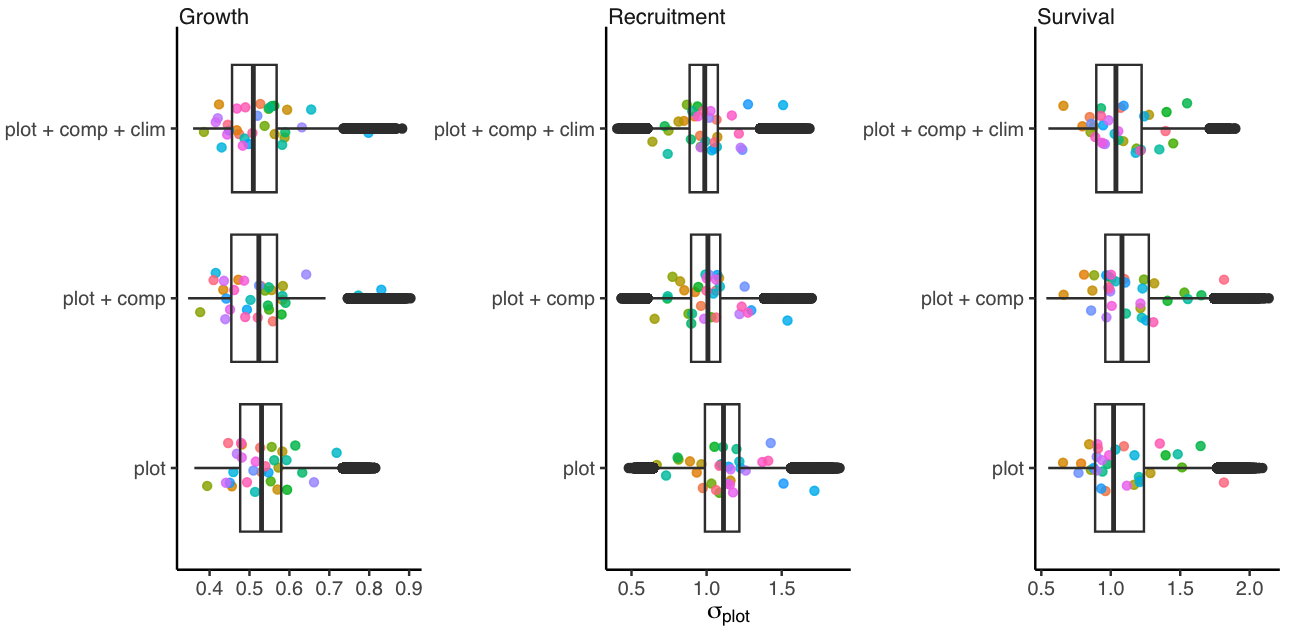
\includegraphics{manuscript/figs/supp1_1.png}
\caption[{Boxplot showing the change in the posterior distribution of
the parameter \(\sigma_{plot}\) across the 31 tree species between the
competing models.}]{Boxplot showing the change in the posterior
distribution of the parameter \(\sigma_{plot}\) across the 31 tree
species between the competing models. For each growth, survival, and
recruitment vital rate, the simplest model (plot random effects only)
increases in complexity with the addition of fixed size, competition,
and climate covariates. Each colored dot represents the species' average
posterior distribution.}
\label{fig:par_var_ch2}
\end{figure}
}

\hypertarget{model-predictive-accuracy}{%
\subsection{Model predictive accuracy}\label{model-predictive-accuracy}}

We used pseudo \(R^2\) and MSE metrics derived from comparing observed
and predicted values to evaluate the predictive accuracy of growth and
recruitment demographic rates. Higher \(R^2\) values and lower MSE
indicate better overall model accuracy. The Figures \ref{fig:R2} and
\ref{fig:MSE} compare the growth and recruitment models using \(R^2\)
and MSE, respectively.\\

\hypertarget{fig:R2}{%
\begin{figure}
\centering
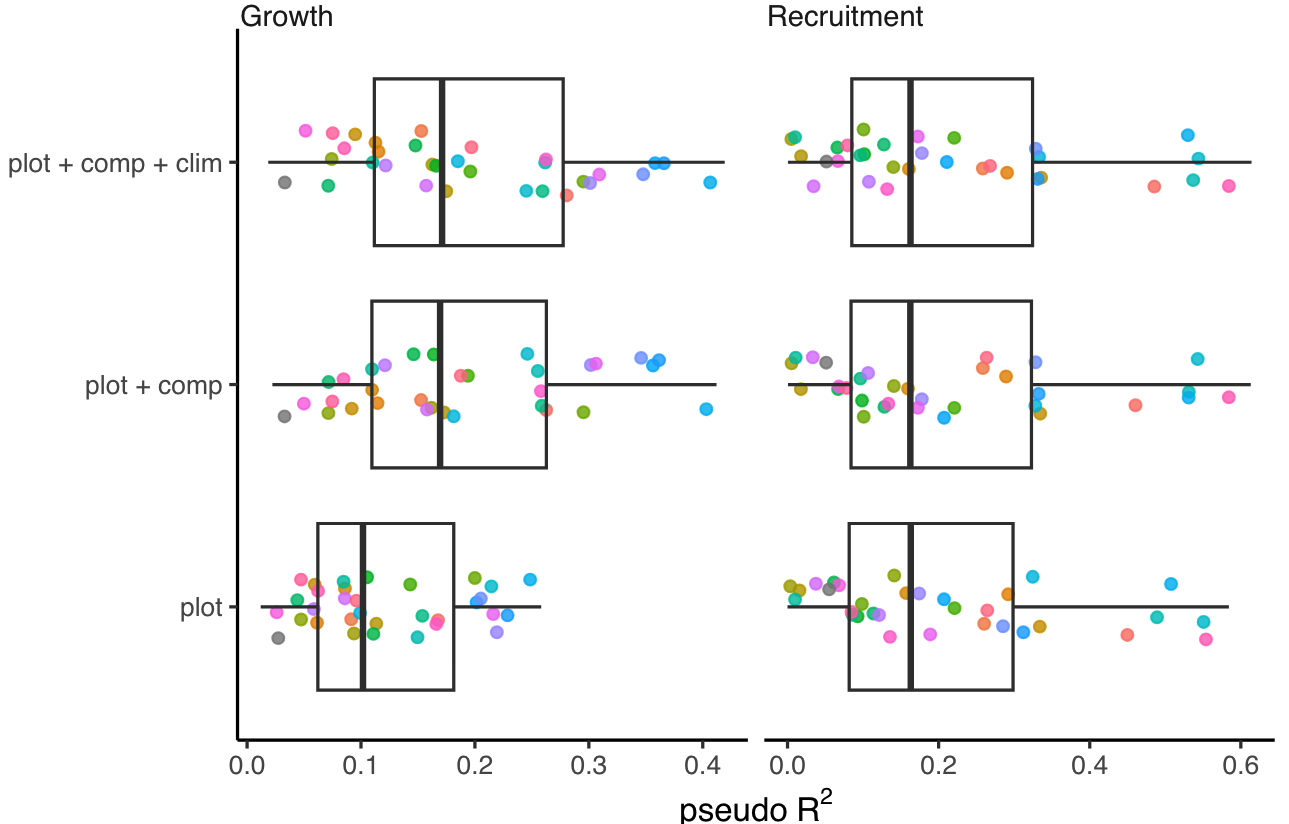
\includegraphics{manuscript/figs/supp1_2.png}
\caption[{Posterior distribution of pseudo \(R^2\) across the 31 tree
species between the competing models.}]{Posterior distribution of pseudo
\(R^2\) across the 31 tree species between the competing models. For
each growth, survival, and recruitment vital rate, the simplest model
(plot random effects only) increases in complexity with the addition of
fixed competition and climate covariates. Each colored dot represents
the species' average posterior distribution.}
\label{fig:R2}
\end{figure}
}

\hypertarget{fig:MSE}{%
\begin{figure}
\centering
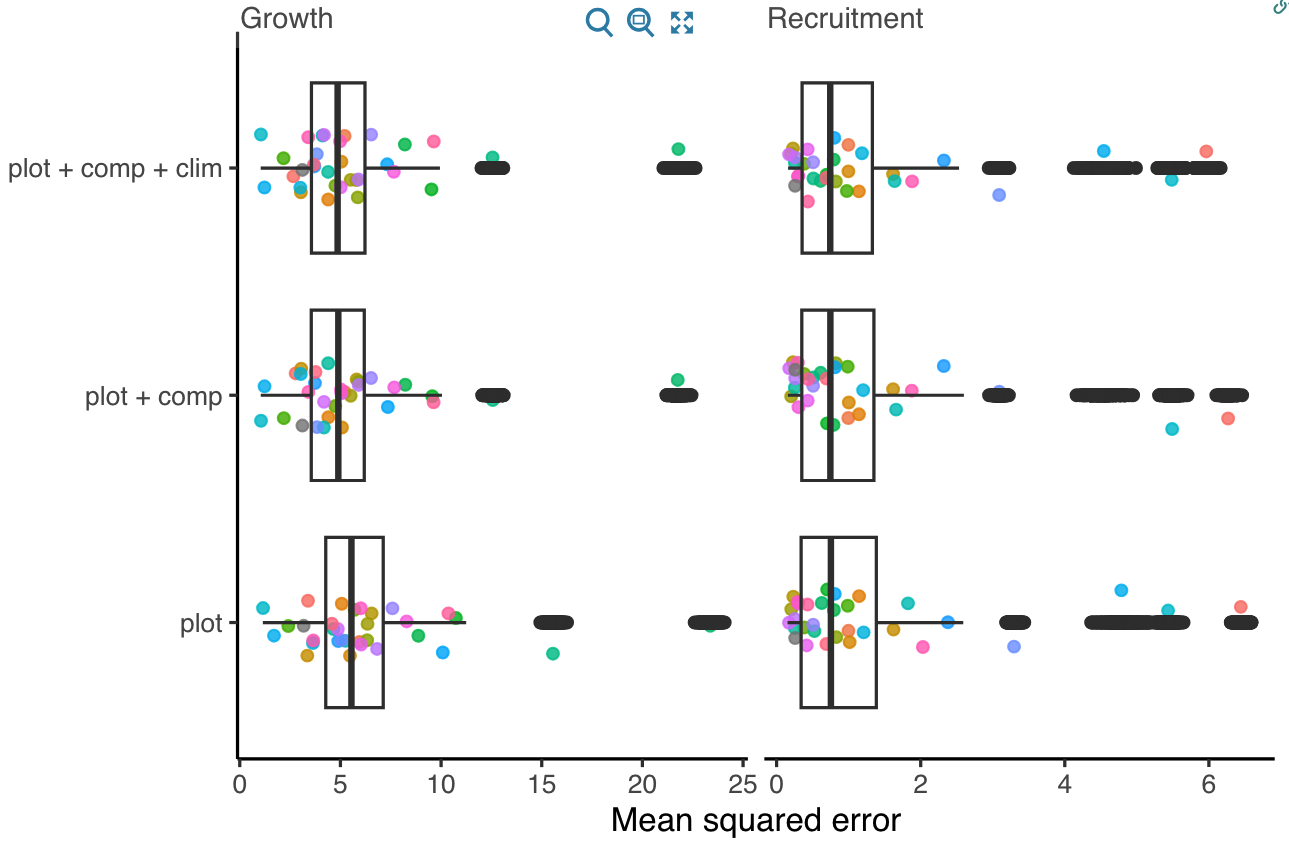
\includegraphics{manuscript/figs/supp1_3.png}
\caption[{Posterior distribution of Mean Squared Error (MSE) across the
31 tree species as models become more complex.}]{Posterior distribution
of Mean Squared Error (MSE) across the 31 tree species as models become
more complex.}
\label{fig:MSE}
\end{figure}
}

We used three complementary metrics for the survival model to assess
model predictions. While the accuracy of classification models is often
evaluated through the fraction of correct predictions, this measure can
be misleading for unbalanced datasets such as mortality, where dead
events are rare. To address this issue, we calculated sensitivity, which
measures the percentage of dead trees correctly identified as dead (true
positives). We also computed specificity, which measures the percentage
of live trees correctly identified as alive (true negatives). The
combination of sensitivity and specificity allows us to calculate
corrected accuracy, considering the unbalanced accuracy predictions of
positive and negative events (Figure \ref{fig:Acc}).\\

\hypertarget{fig:Acc}{%
\begin{figure}
\centering
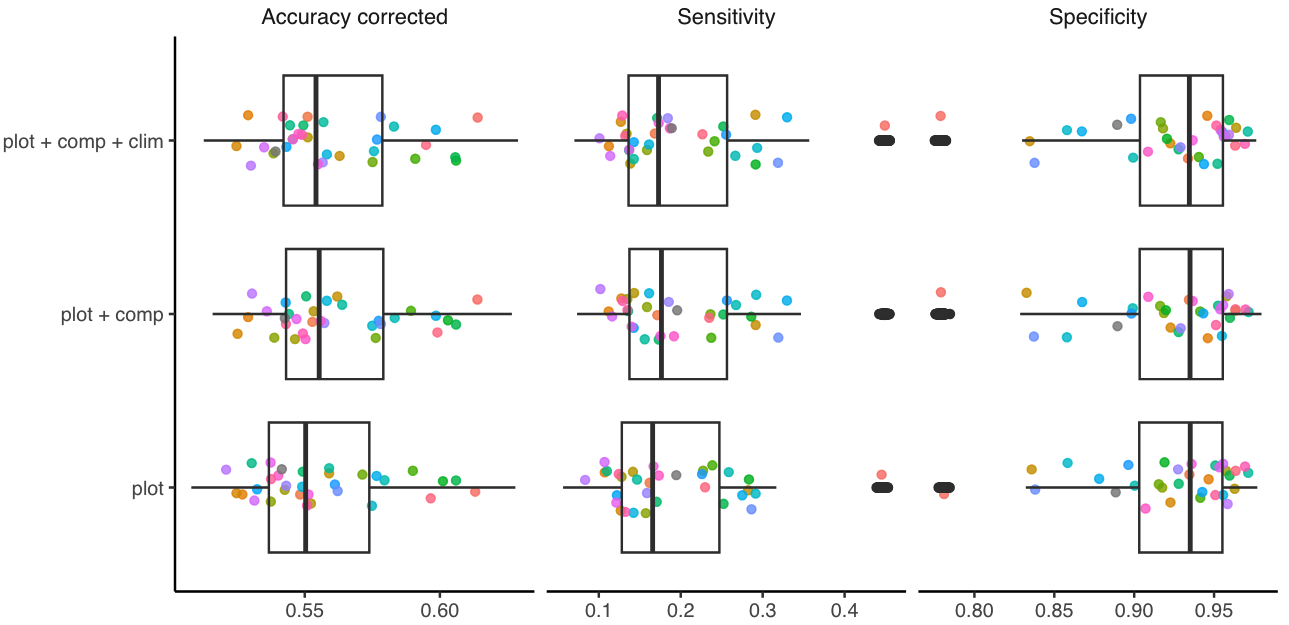
\includegraphics{manuscript/figs/supp1_4.png}
\caption[{Comparing the posterior distribution of sensitivity,
specificity, and accuracy across the 31 tree species between the
competing models.}]{Comparing the posterior distribution of sensitivity,
specificity, and accuracy across the 31 tree species between the
competing models. Each colored dot represents the species' average
posterior distribution.}
\label{fig:Acc}
\end{figure}
}

\hypertarget{leave-one-out-cross-validation}{%
\subsection{Leave-one-out
cross-validation}\label{leave-one-out-cross-validation}}

Finally, we evaluated the competing models using the LOO-CV metric
(Figure \ref{fig:loo}), where models are compared based on the
difference in the expected log pointwise predictive density
(ELPD\_diff). In cases involving multiple models, the difference is
calculated relative to the model with highest ELPD
\citep{vehtari2017practical}. Consequently, the model with ELPD\_diff
equal to zero is defined as the best model. In contrast, the performance
of the other models is assessed based on their deviation from the
reference model in pointwise predictive cross-validation. Given the
large number of observations in the dataset, we approximated LOO-CV
using PSIS-LOO and subsampling. For each species, we approximated LOO-CV
by sampling one-fifth of the total number of observations.\\

\hypertarget{fig:loo}{%
\begin{figure}
\centering
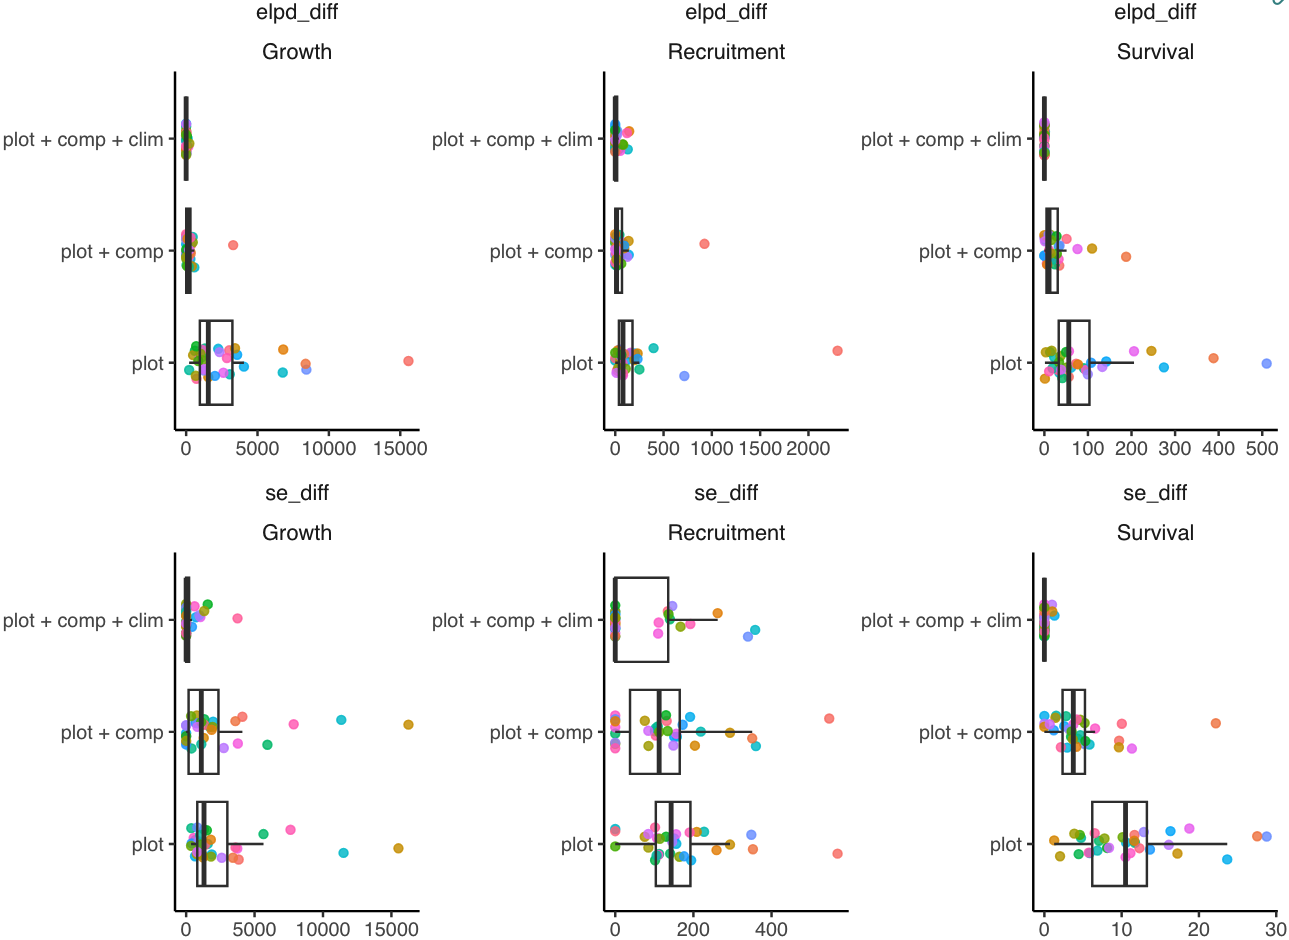
\includegraphics{manuscript/figs/supp1_5.png}
\caption[{Boxplot shows the LOO-CV compare between the competing models
based on the expected log pointwise predictive density (ELPD\_diff)
difference across the 31 tree species.}]{Boxplot shows the LOO-CV
compare between the competing models based on the expected log pointwise
predictive density (ELPD\_diff) difference across the 31 tree species.
The sd\_diff is the standard error of the ELPD difference between the
model and the reference model (ELPD\_diff equal to zero).}
\label{fig:loo}
\end{figure}
}

\hypertarget{size-effect-in-survival}{%
\subsection{Size effect in survival}\label{size-effect-in-survival}}

We initially incorporated the size effect into the survival models due
to the structured-population approach. However, we observed that the
effect of size on mortality probability was generally weak and variable
among species, with no clear pattern of increased mortality probability
with larger individual size. All models that included the size effect
performed worse than the null model, which contained only plot random
effects (Figure \ref{fig:loo_mort}).\\

\hypertarget{fig:loo_mort}{%
\begin{figure}
\centering
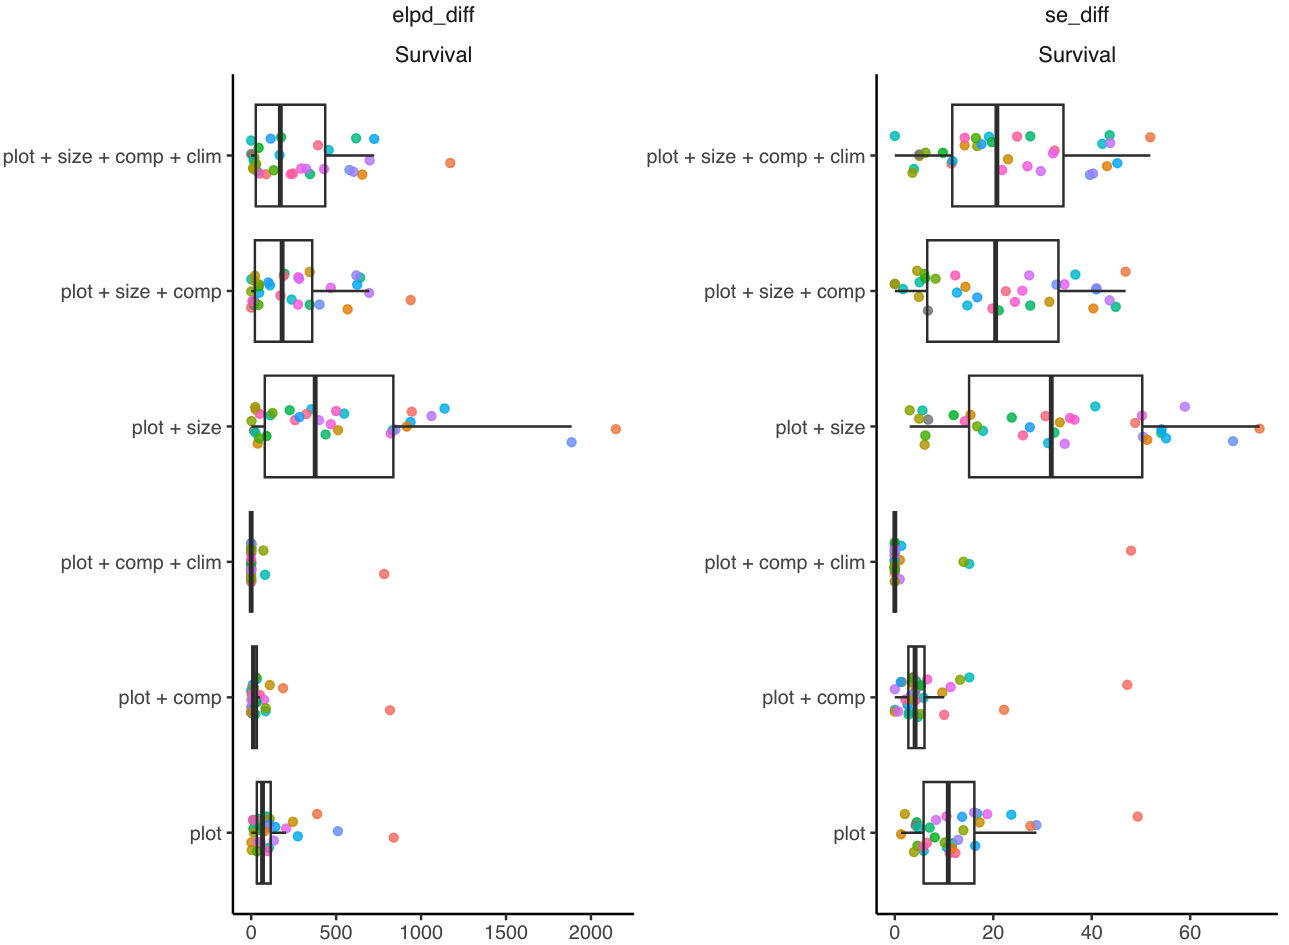
\includegraphics{manuscript/figs/supp1_6.png}
\caption[{Boxplot shows the LOO-CV compare between the competing models
based on the expected log pointwise predictive density (ELPD\_diff)
difference across the 31 tree species.}]{Boxplot shows the LOO-CV
compare between the competing models based on the expected log pointwise
predictive density (ELPD\_diff) difference across the 31 tree species.
The sd\_diff is the standard error of the ELPD difference between the
model and the reference model (ELPD\_diff equal to zero).}
\label{fig:loo_mort}
\end{figure}
}

\hypertarget{conclusion}{%
\subsection{Conclusion}\label{conclusion}}

Our analysis revealed that incorporating competition into the growth,
survival, and recruitment models proved more effective in gaining
individual-level information than climate variables. The parameter
\(\sigma_{plot}\), interpreted as spatial heterogeneity, was lowest in
the growth model, followed by recruitment and survival. As the models
became more complex with the inclusion of covariates, recruitment
exhibited the most significant reduction in spatial variance, followed
by growth, with no clear pattern in the case of survival.\\

Regarding predictive performance, competition contributed more to the
overall predictive capacity (\(R^2\), MSE, and corrected accuracy) in
the growth and survival models compared to climate variables. Although
recruitment had the largest reduction in \(\sigma_{plot}\), it had
minimal impact on prediction accuracy.\\

Finally, the LOO-CV indicates a clear trend where the complete model
featuring plot random effects, competition, and climate covariates
outperformed the other competing models. Furthermore, the absolute value
of the ELPD shows that the growth model gained the most information from
including covariates, followed by recruitment and survival models.
Consequently, we selected the complete model with plot random effects,
competition, and climate covariates as the preferred model for further
analysis.\\

\newpage

\hypertarget{supplementary-material-2}{%
\section{Supplementary Material 2}\label{supplementary-material-2}}

\hypertarget{tbl:variability_impl_mech}{%
\begin{longtable}{lrrr}
\caption{List of species and their frequency across the dataset.}
\label{tbl:variability_impl_mech}
\endfirsthead
\endhead
  \toprule
    Species & Number of
    plots & Number of
    individual & Number of
    observation \\
    \midrule\addlinespace[2.5pt]
    \emph{Acer rubrum} & 13149 & 96739 & 235408 \\
    \emph{Abies balsamea} & 11932 & 247737 & 521565 \\
    \emph{Betula papyrifera} & 9508 & 78049 & 203500 \\
    \emph{Picea mariana} & 7869 & 186491 & 454246 \\
    \emph{Acer saccharum} & 7403 & 71961 & 184641 \\
    \emph{Picea glauca} & 5889 & 27641 & 65626 \\
    \emph{Populus tremuloides} & 5876 & 56010 & 127115 \\
    \emph{Betula alleghaniensis} & 5624 & 28872 & 73116 \\
    \emph{Quercus rubra} & 4549 & 18272 & 46341 \\
    \emph{Quercus alba} & 4200 & 20376 & 51466 \\
    \emph{Fagus grandifolia} & 3819 & 21784 & 51764 \\
    \emph{Prunus serotina} & 3730 & 12178 & 26464 \\
    \emph{Thuja occidentalis} & 3230 & 51312 & 125811 \\
    \emph{Pinus strobus} & 3165 & 15638 & 38470 \\
    \emph{Fraxinus americana} & 2885 & 8942 & 21501 \\
    \emph{Quercus velutina} & 2722 & 10068 & 23298 \\
    \emph{Tsuga canadensis} & 2604 & 17914 & 45198 \\
    \emph{Nyssa sylvatica} & 2436 & 6275 & 15785 \\
    \emph{Quercus stellata} & 2279 & 14707 & 32102 \\
    \emph{Picea rubens} & 2190 & 16580 & 41674 \\
    \emph{Liquidambar styraciflua} & 2154 & 11655 & 29671 \\
    \emph{Fraxinus pennsylvanica} & 2149 & 9048 & 20588 \\
    \emph{Tilia americana} & 2059 & 8415 & 21412 \\
    \emph{Pinus banksiana} & 2057 & 34122 & 75372 \\
    \emph{Populus grandidentata} & 2015 & 13759 & 29358 \\
    \emph{Fraxinus nigra} & 1951 & 12633 & 31156 \\
    \emph{Liriodendron tulipifera} & 1912 & 8580 & 21071 \\
    \emph{Carya tomentosa} & 1636 & 3897 & 10590 \\
    \emph{Carya glabra} & 1622 & 4002 & 9916 \\
    \emph{Quercus prinus} & 1590 & 11000 & 27554 \\
    \emph{Juniperus virginiana} & 1571 & 9474 & 21400 \\
  \bottomrule
\end{longtable}
}

\newpage

\hypertarget{fig:figsupp1_ch2}{%
\begin{figure}
\centering
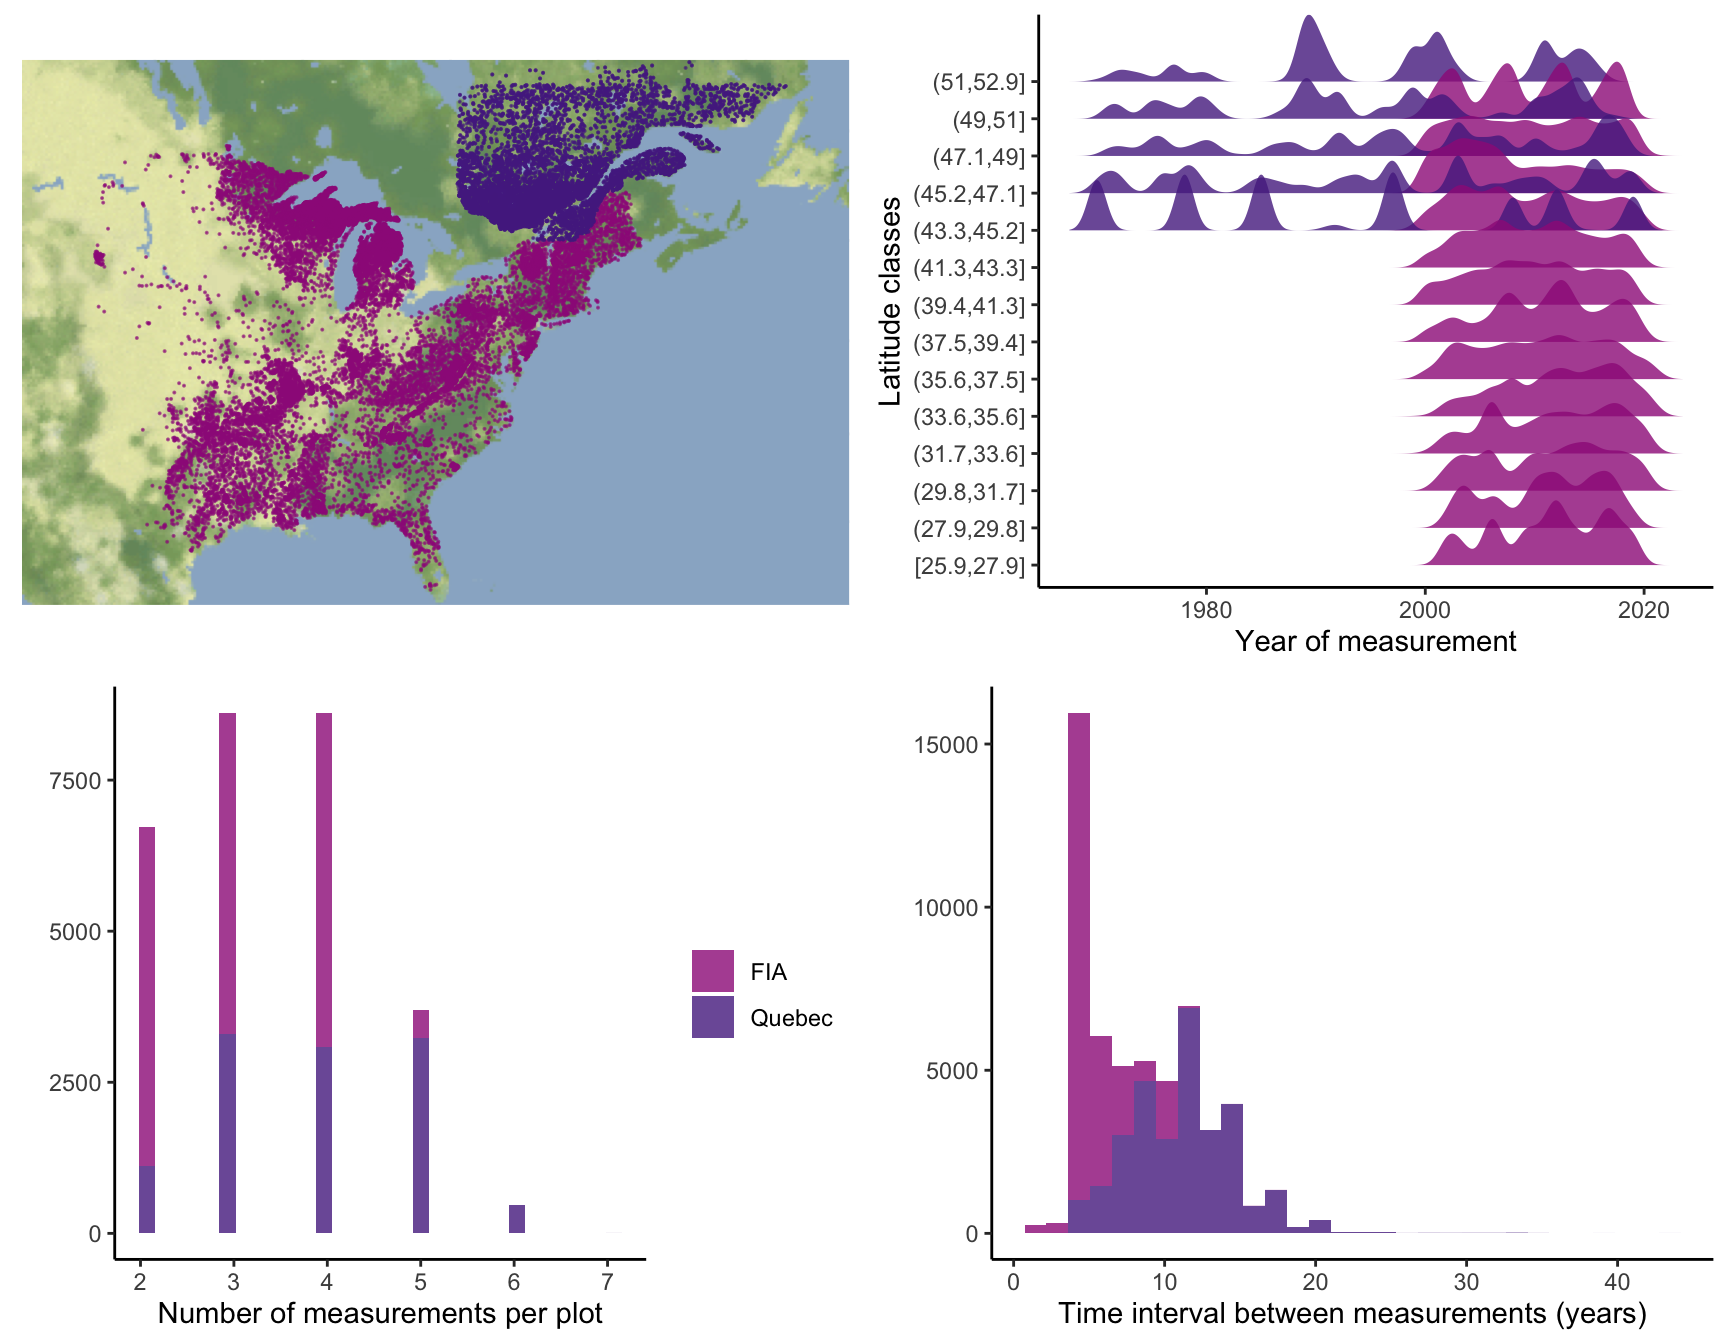
\includegraphics{manuscript/figs/fig-plotCoverage-1.png}
\caption[{Spatial (top left) and temporal (top right) coverage of the
dataset incorporating data from the USA and Quebec.}]{Spatial (top left)
and temporal (top right) coverage of the dataset incorporating data from
the USA and Quebec. The top right panel shows the distribution of
observations per class of latitude for the 31 species used in this
study.}
\label{fig:figsupp1_ch2}
\end{figure}
}

\newpage

\hypertarget{fig:figsupp2_ch2}{%
\begin{figure}
\centering
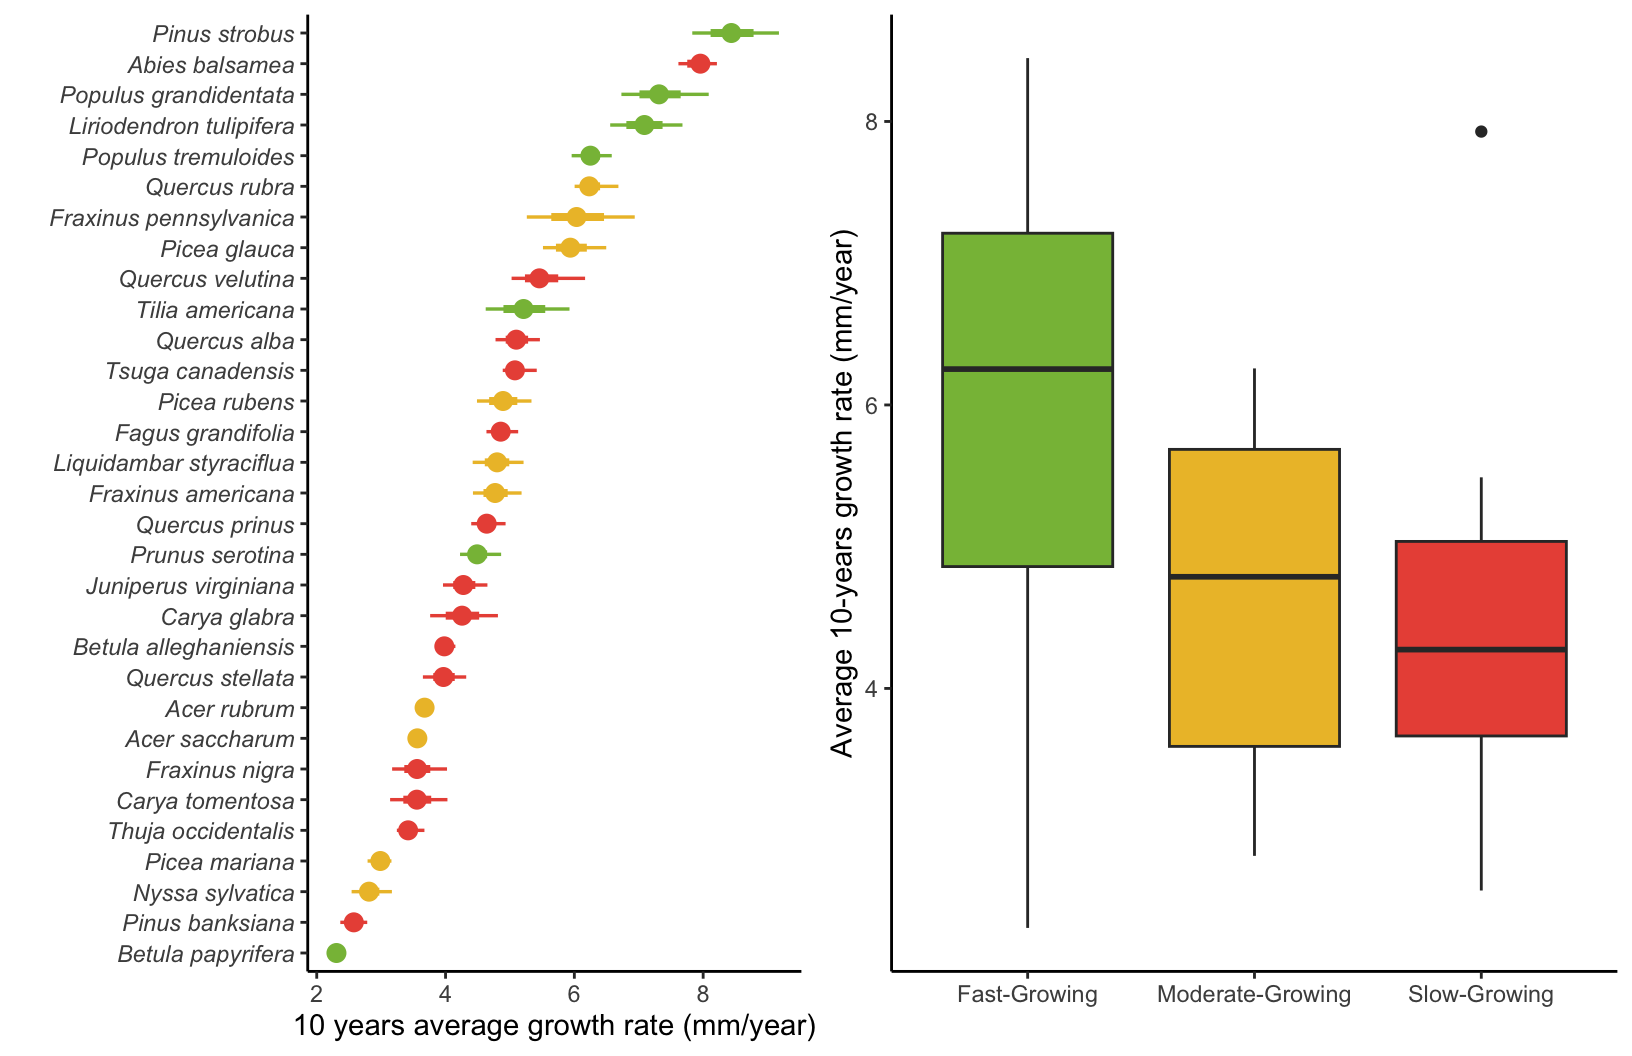
\includegraphics{manuscript/figs/fig-intGrowth-1.png}
\caption[{Posterior distribution for the intercept of the growth model
using the 10-year average growth rate.}]{Posterior distribution for the
intercept of the growth model using the 10-year average growth rate.
Species are classified by their general growth trait following
\citet{burns1990silvics}.}
\label{fig:figsupp2_ch2}
\end{figure}
}

\newpage

\hypertarget{fig:figsupp3_ch2}{%
\begin{figure}
\centering
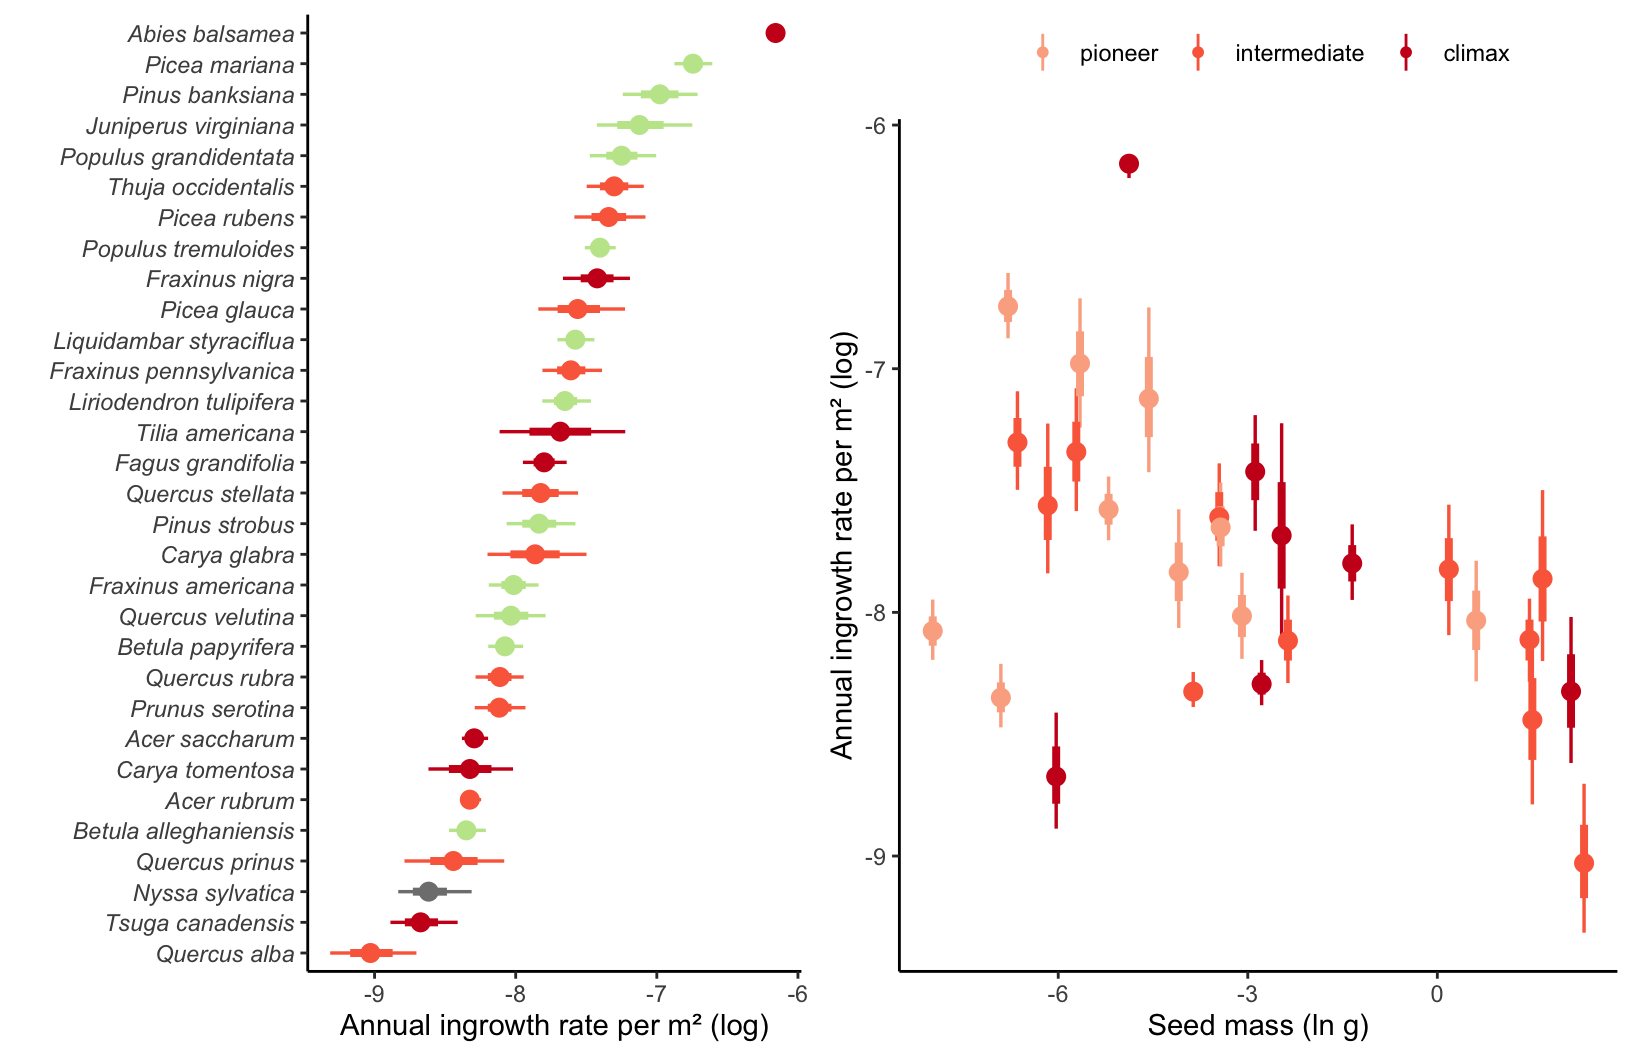
\includegraphics{manuscript/figs/fig-intcerpt_ingrowth-1.png}
\caption[{Posterior distribution for the intercept of the ingrwoth model
for the number of individuals that ingress the population per year per
\(m^2\) in function seed mass \citep{diaz2022}.}]{Posterior distribution
for the intercept of the ingrwoth model for the number of individuals
that ingress the population per year per \(m^2\) in function seed mass
\citep{diaz2022}. Species are classified by their successional status
following \citet{burns1990silvics}.}
\label{fig:figsupp3_ch2}
\end{figure}
}

\newpage

\hypertarget{fig:figsupp4_ch2}{%
\begin{figure}
\centering
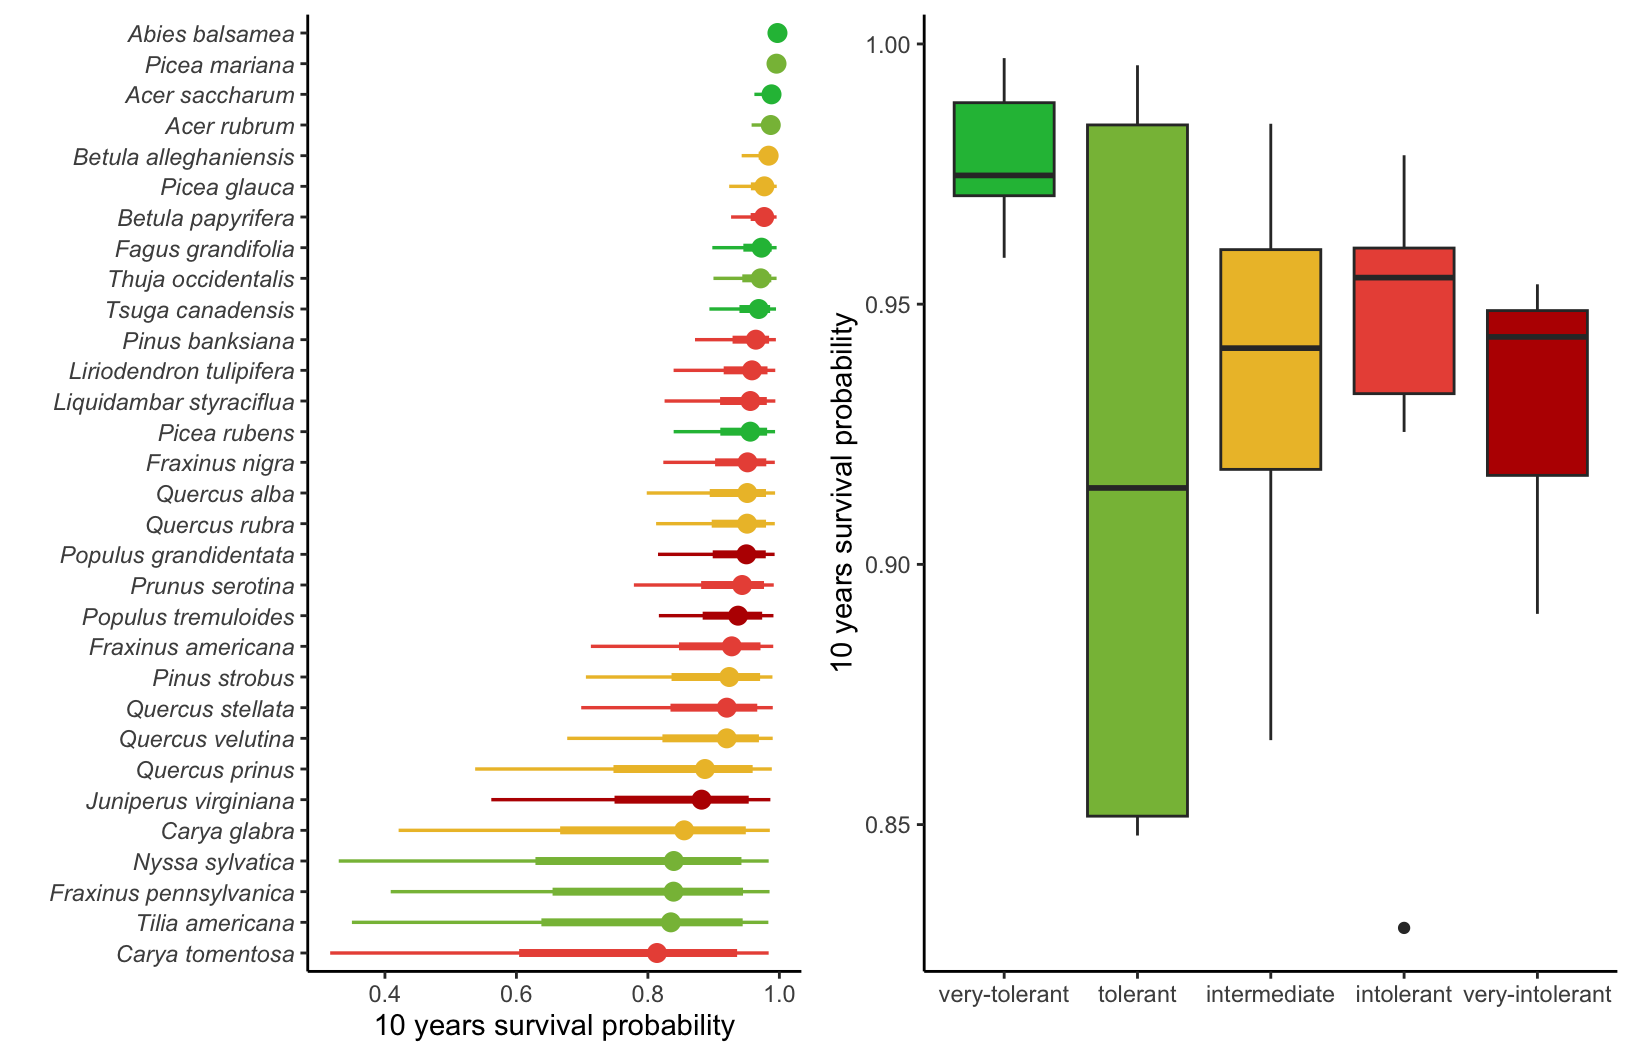
\includegraphics{manuscript/figs/fig-intcerpt_ingP-1.png}
\caption[{Posterior distribution for the intercept of the annual
survival probability for the ingrowth model.}]{Posterior distribution
for the intercept of the annual survival probability for the ingrowth
model. Species are classified by their shade tolerance trait following
\citet{burns1990silvics}.}
\label{fig:figsupp4_ch2}
\end{figure}
}

\newpage

\hypertarget{fig:figsupp5_ch2}{%
\begin{figure}
\centering
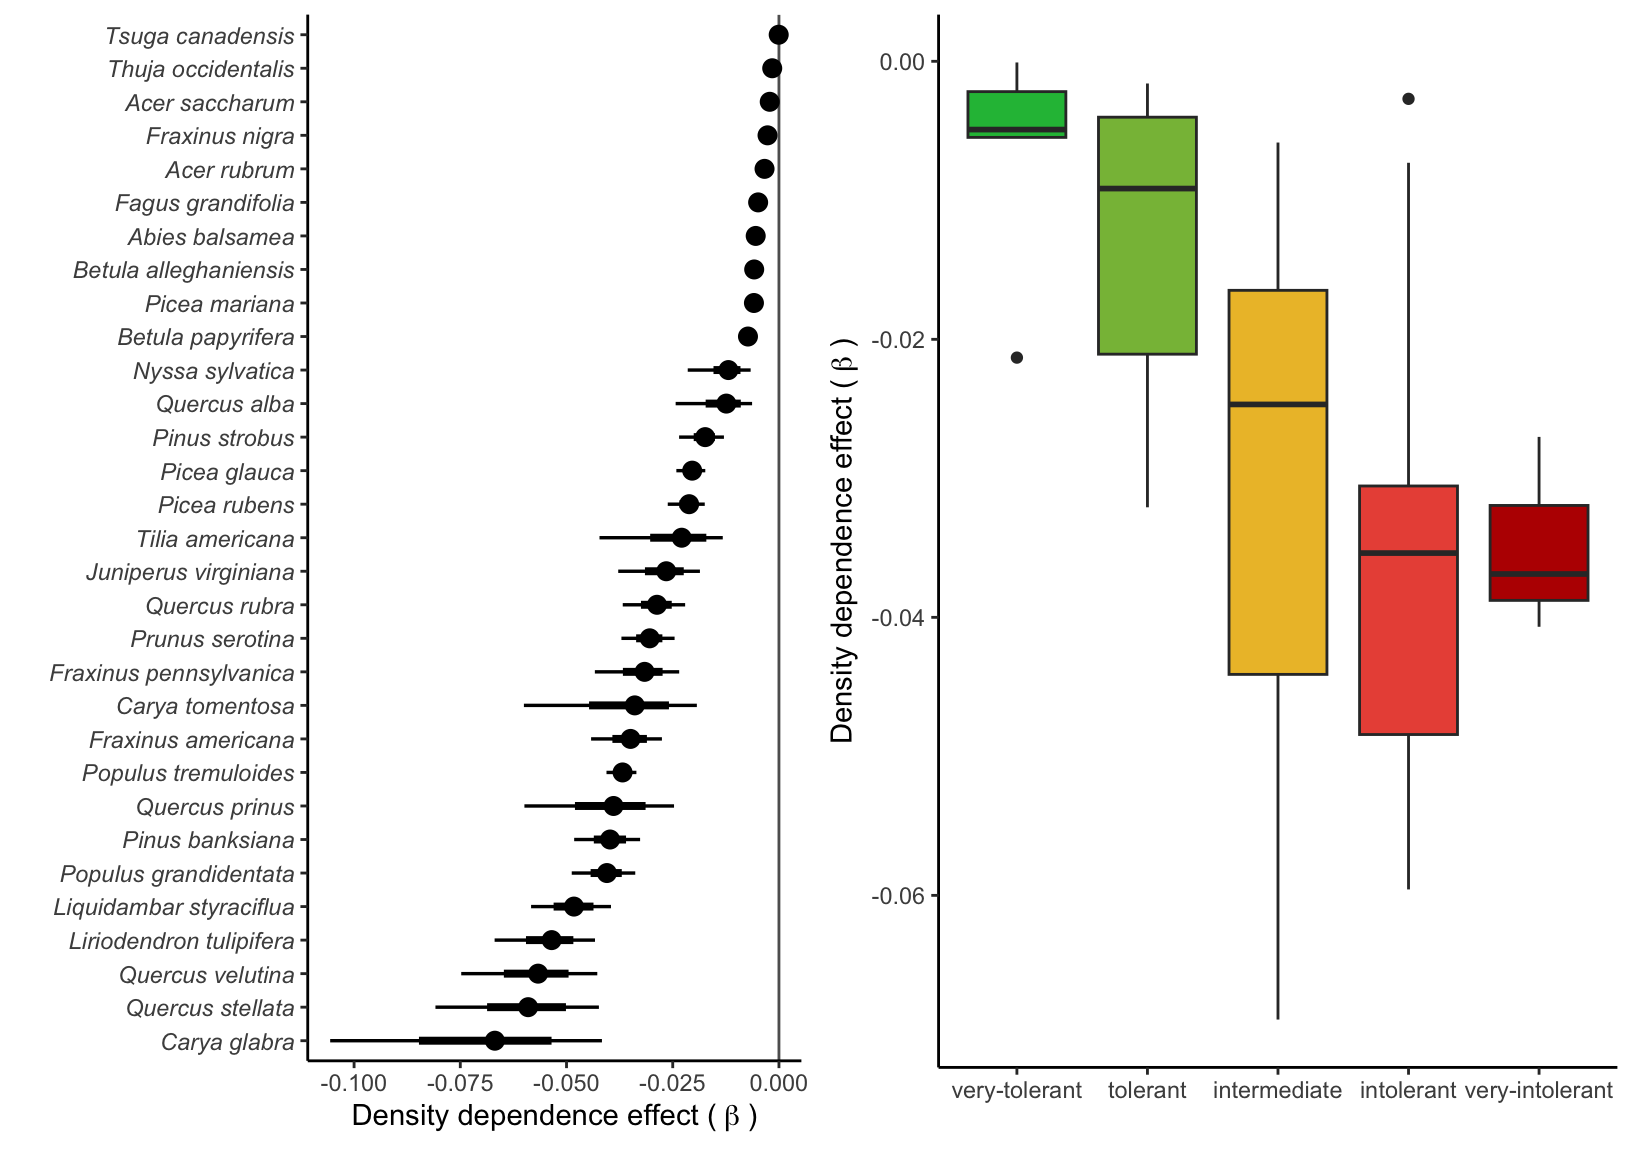
\includegraphics{manuscript/figs/fig-compRec-1.png}
\caption[{Posterior distribution of the density dependence parameter
affecting the annual survival rate of recruitment
individuals.}]{Posterior distribution of the density dependence
parameter affecting the annual survival rate of recruitment individuals.
Species are classified by their shade tolerance trait following
\citet{burns1990silvics}.}
\label{fig:figsupp5_ch2}
\end{figure}
}

\newpage

\hypertarget{fig:figsupp6_ch2}{%
\begin{figure}
\centering
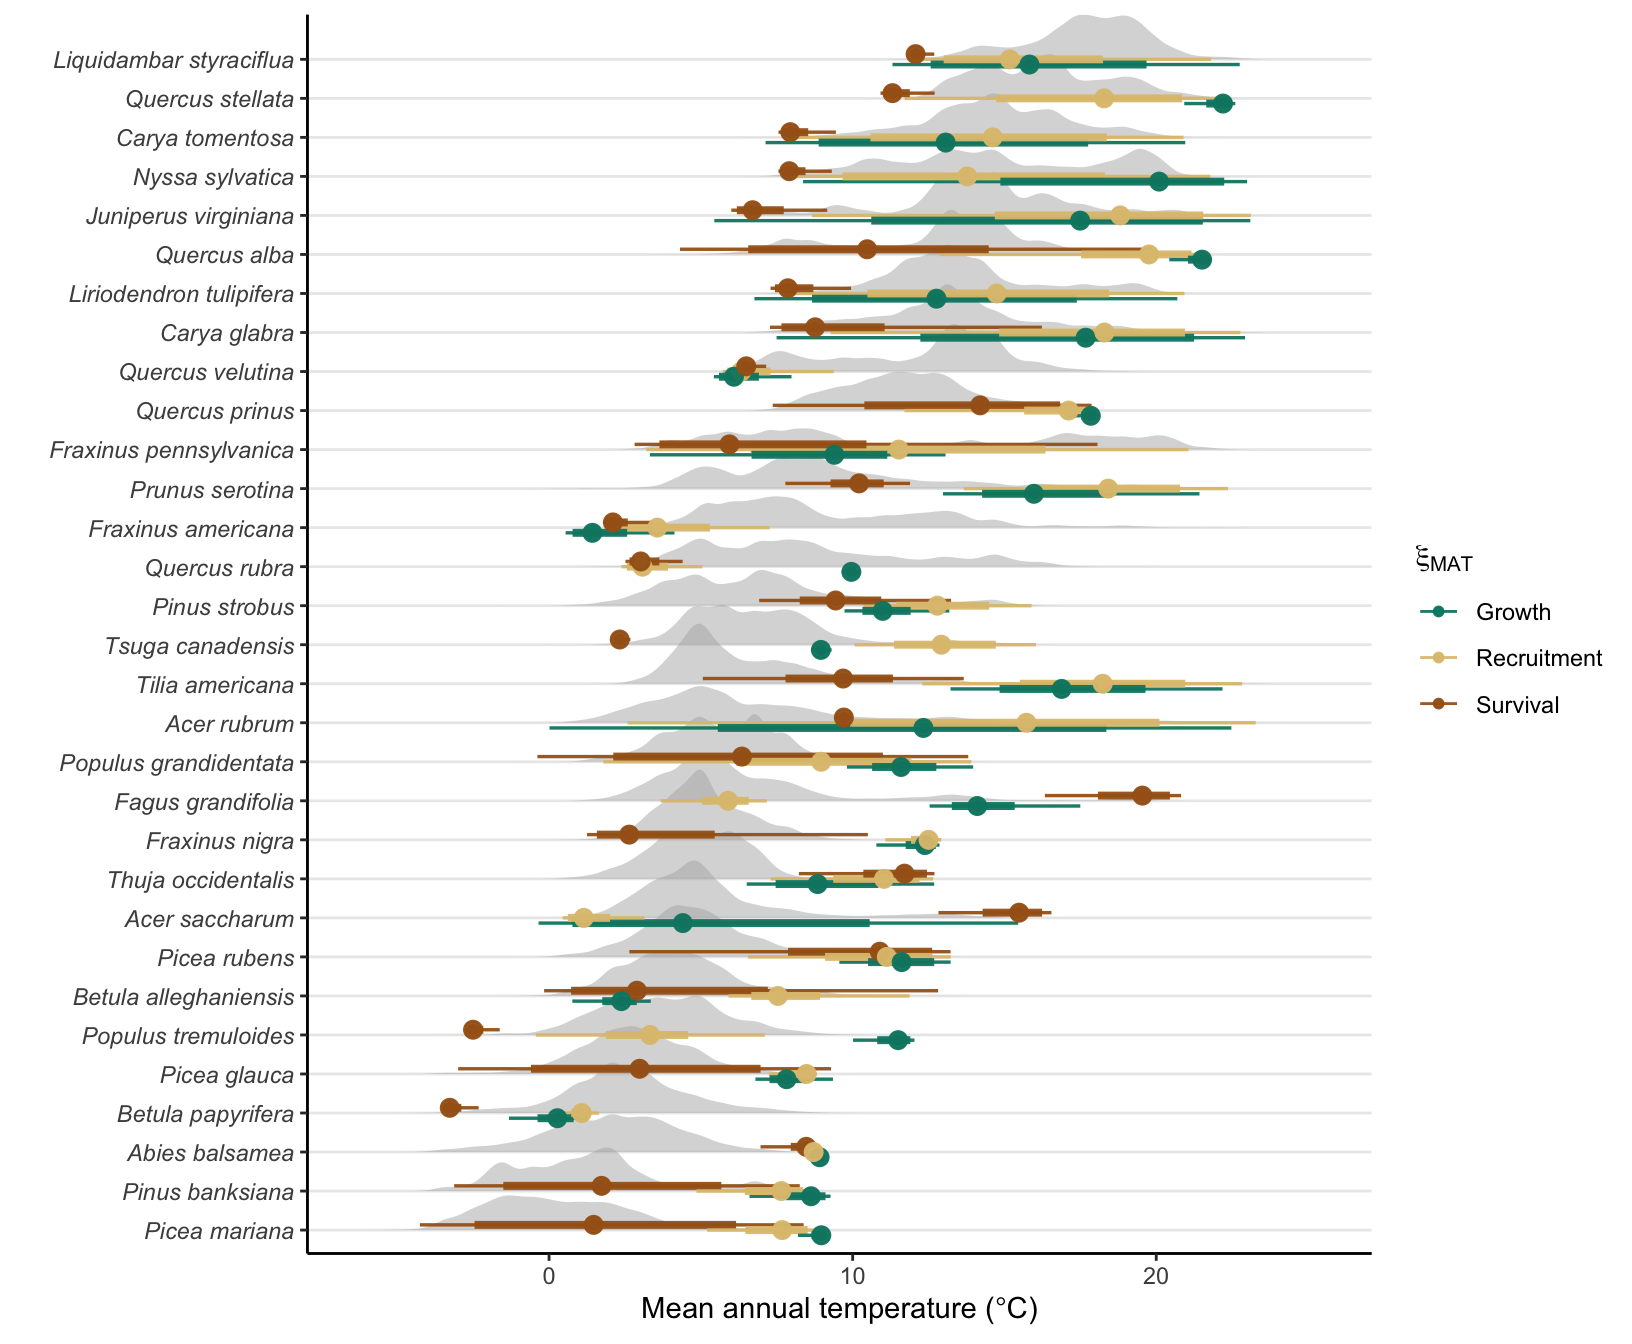
\includegraphics{manuscript/figs/fig-matDist-1.png}
\caption[{Distribution for the optimal annual mean temperature
(\(\xi_{MAT}\)) for growth (green), recruitment (yellow), and survival
(brown).}]{Distribution for the optimal annual mean temperature
(\(\xi_{MAT}\)) for growth (green), recruitment (yellow), and survival
(brown). The gray density plot is the annual mean temperature
distribution among all observed trees across space and time.}
\label{fig:figsupp6_ch2}
\end{figure}
}

\newpage

\hypertarget{fig:figsupp7_ch2}{%
\begin{figure}
\centering
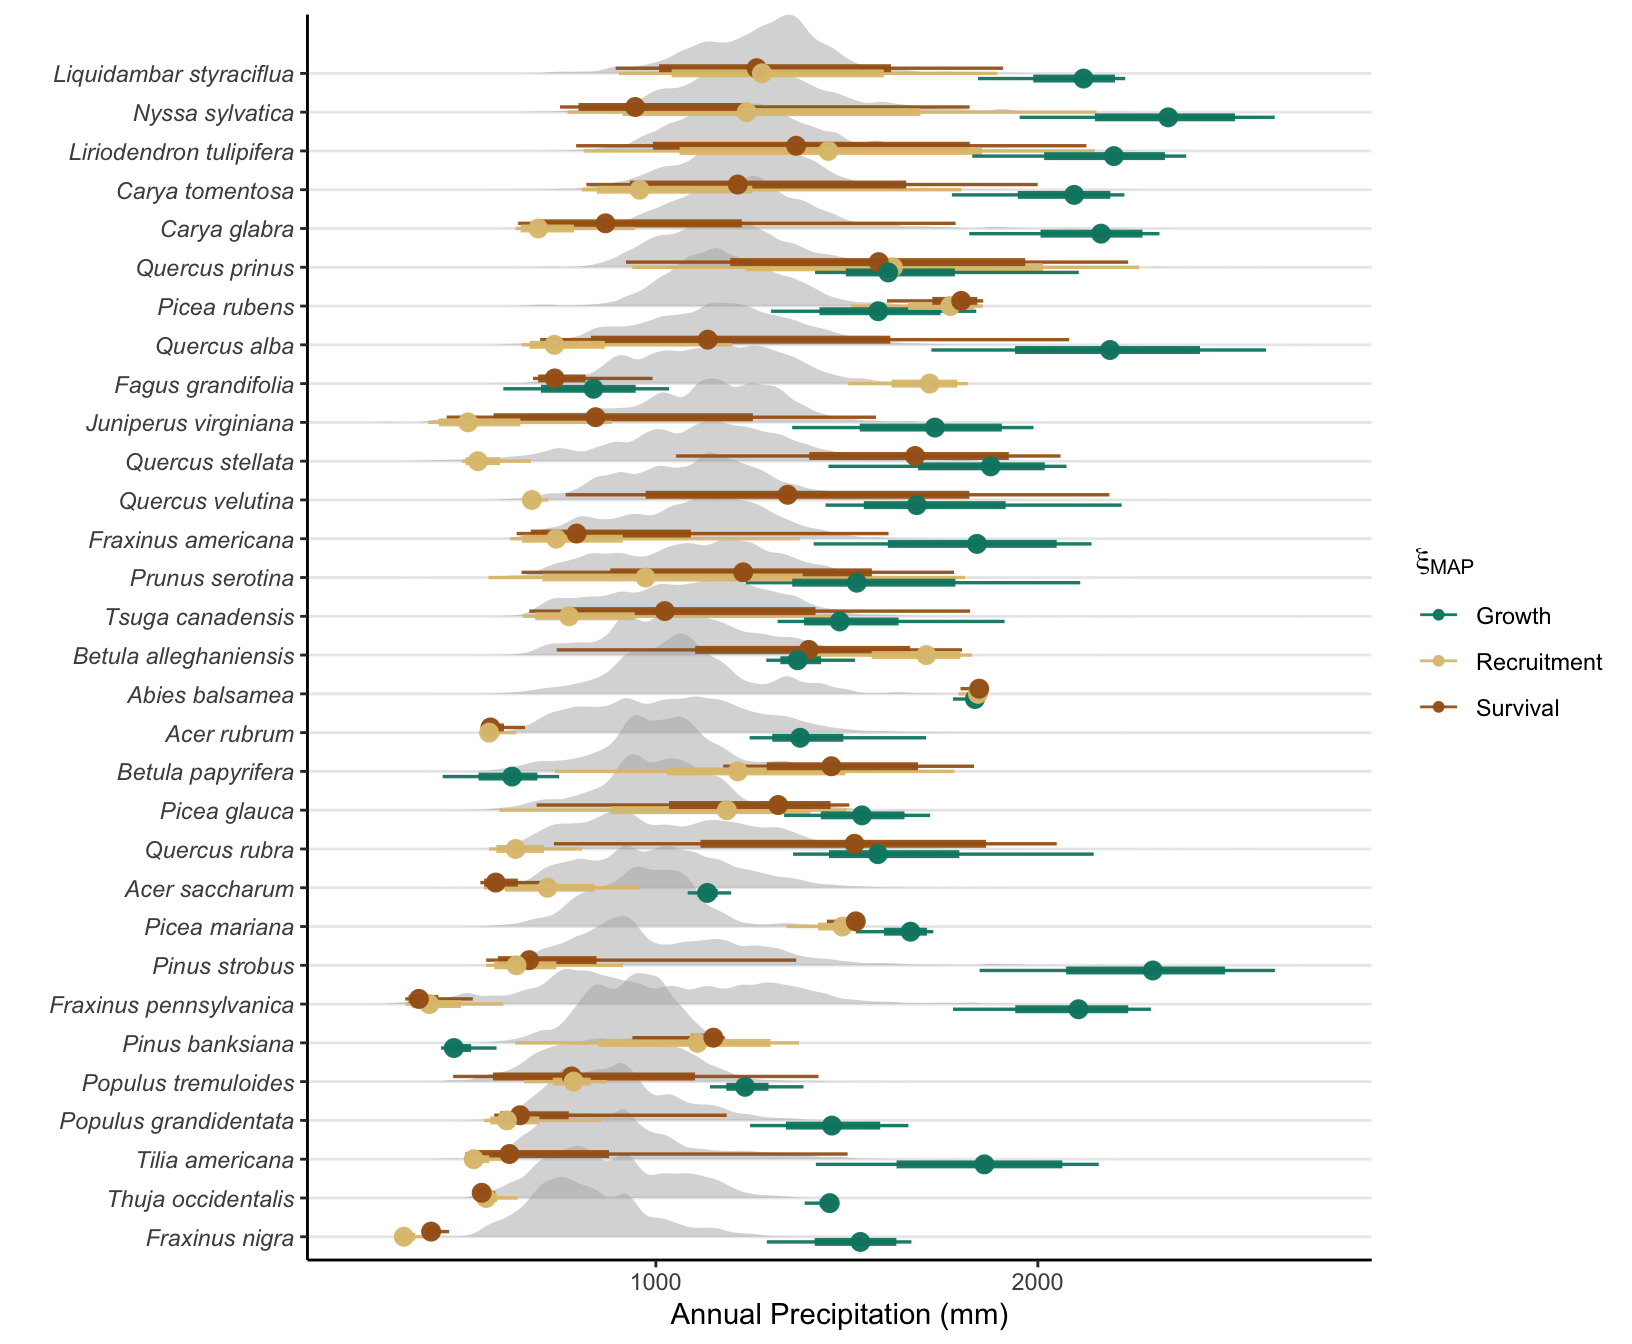
\includegraphics{manuscript/figs/fig-mapDist-1.png}
\caption[{Distribution for the optimal mean annual precipitation
(\(\xi_{MAP}\)) for growth (green), recruitment (yellow), and survival
(brown).}]{Distribution for the optimal mean annual precipitation
(\(\xi_{MAP}\)) for growth (green), recruitment (yellow), and survival
(brown). The density plot in gray is the distribution of annual
precipitation variable among all observed trees across space and time.}
\label{fig:figsupp7_ch2}
\end{figure}
}

\newpage

\hypertarget{fig:figsupp8_ch2}{%
\begin{figure}
\centering
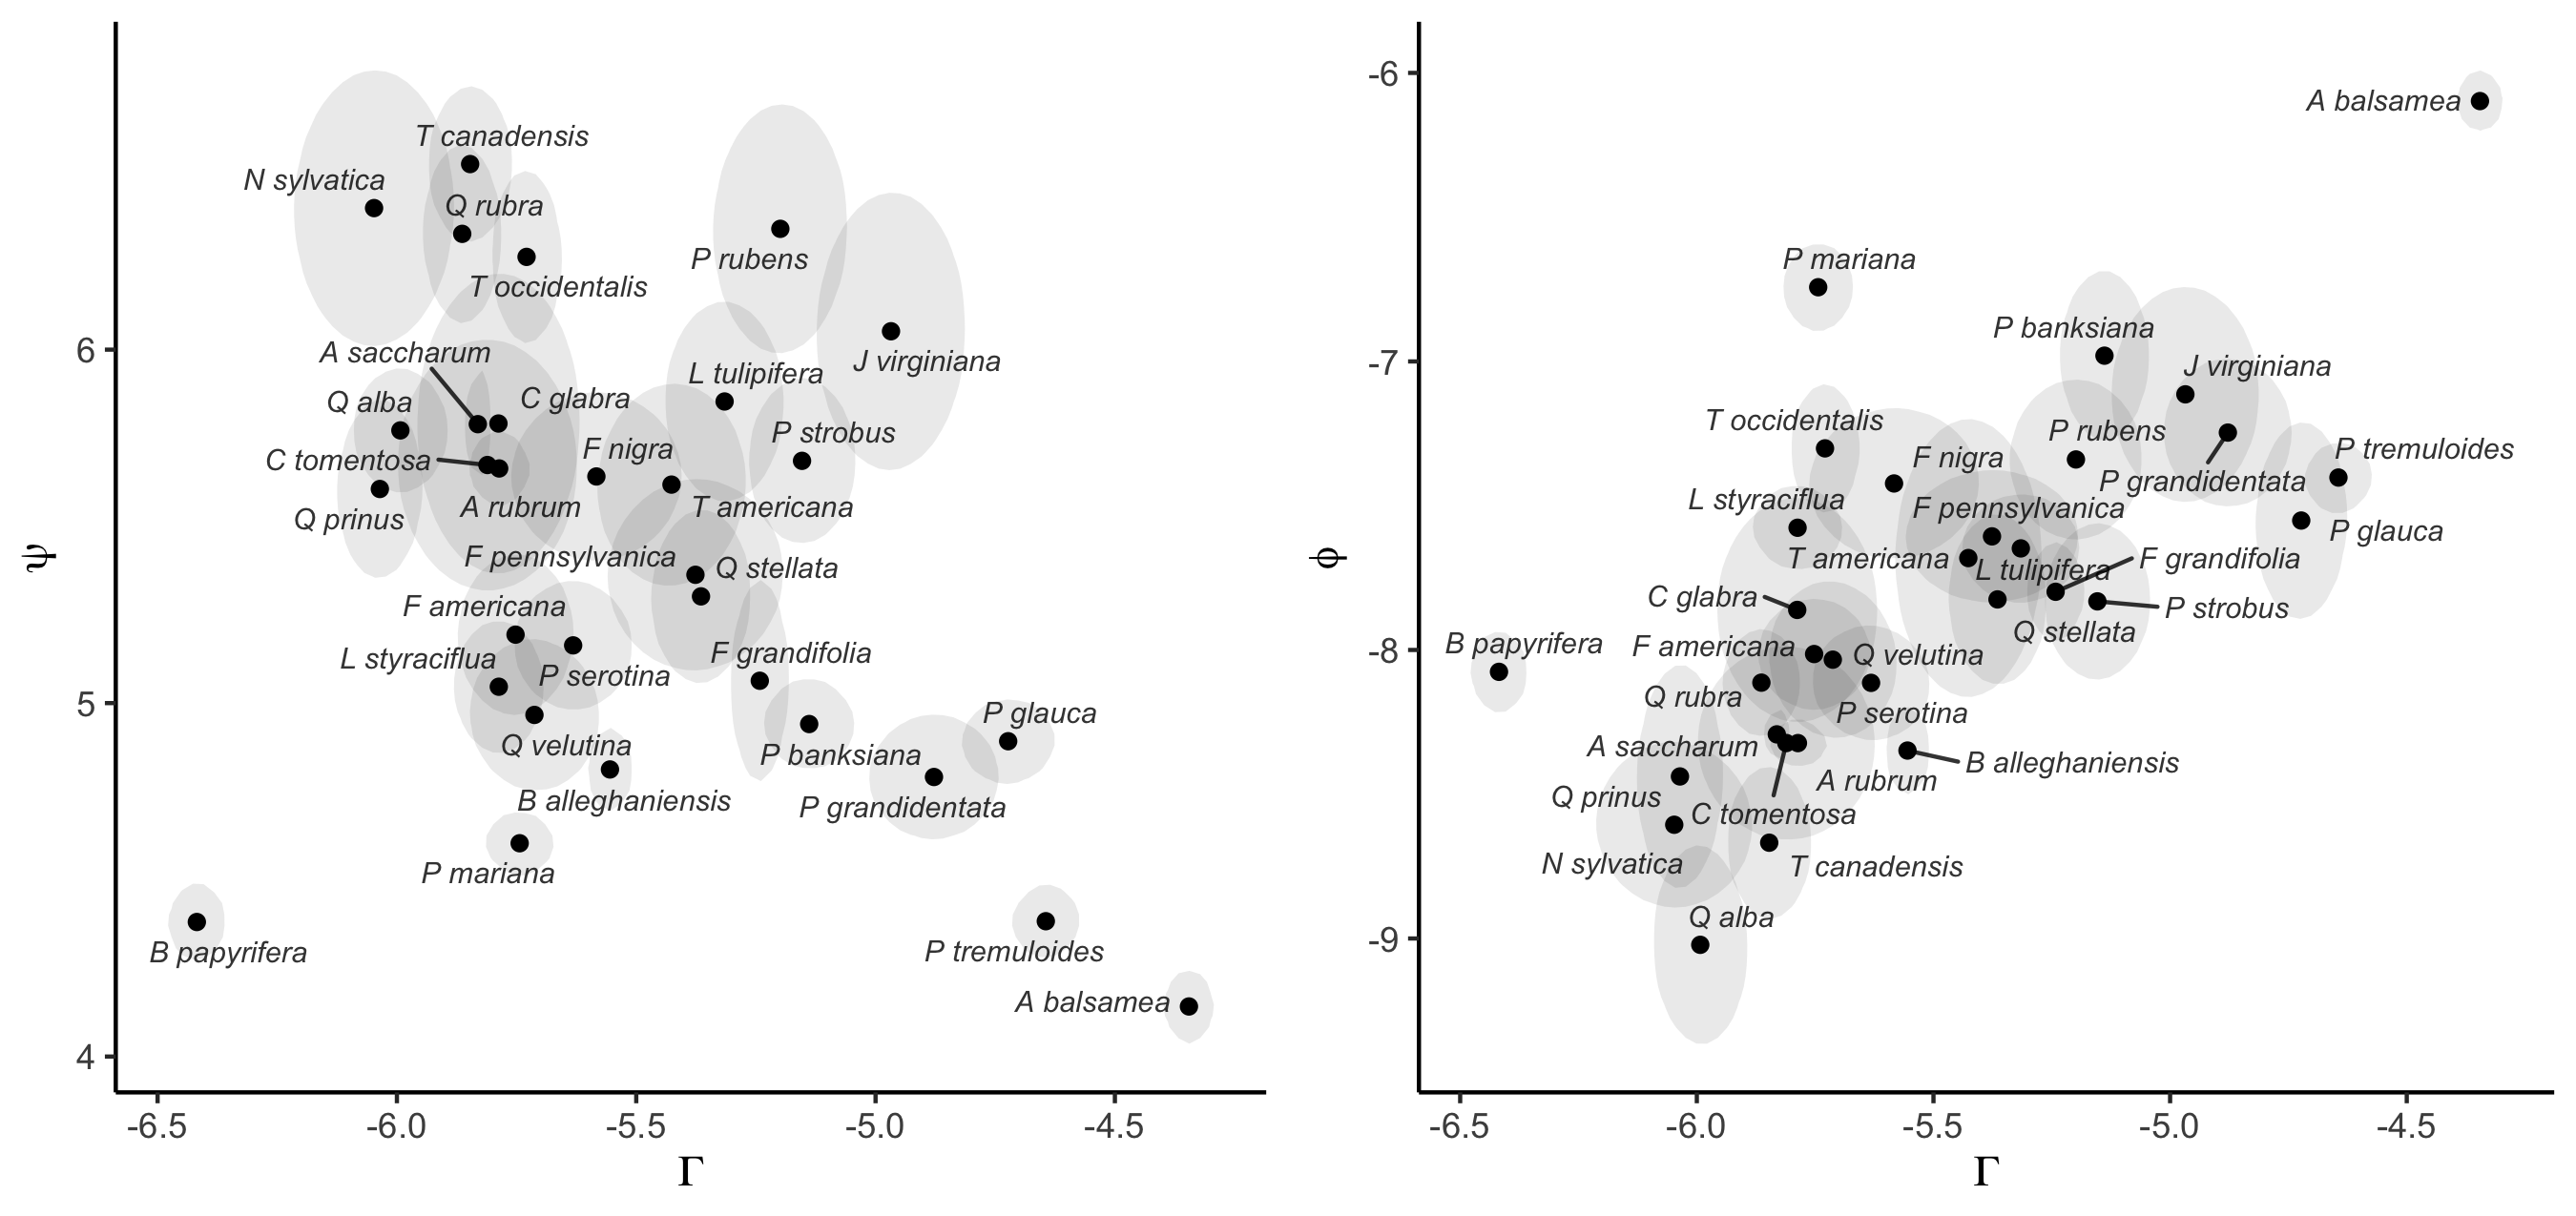
\includegraphics{manuscript/figs/intercept_corr.png}
\caption[{Correlation between (left panel) growth rate (\(\Gamma\)) and
annual survival rate (\(\psi\)) and (right panel) growth rate
(\(\Gamma\)) and annual recruitment rate (\(\phi\)).}]{Correlation
between (left panel) growth rate (\(\Gamma\)) and annual survival rate
(\(\psi\)) and (right panel) growth rate (\(\Gamma\)) and annual
recruitment rate (\(\phi\)). The uncertainty of the parameters is
summarised by a Multivariate Normal Density function with 90\%
probability.}
\label{fig:figsupp8_ch2}
\end{figure}
}

\newpage

\hypertarget{fig:figsupp9_ch2}{%
\begin{figure}
\centering
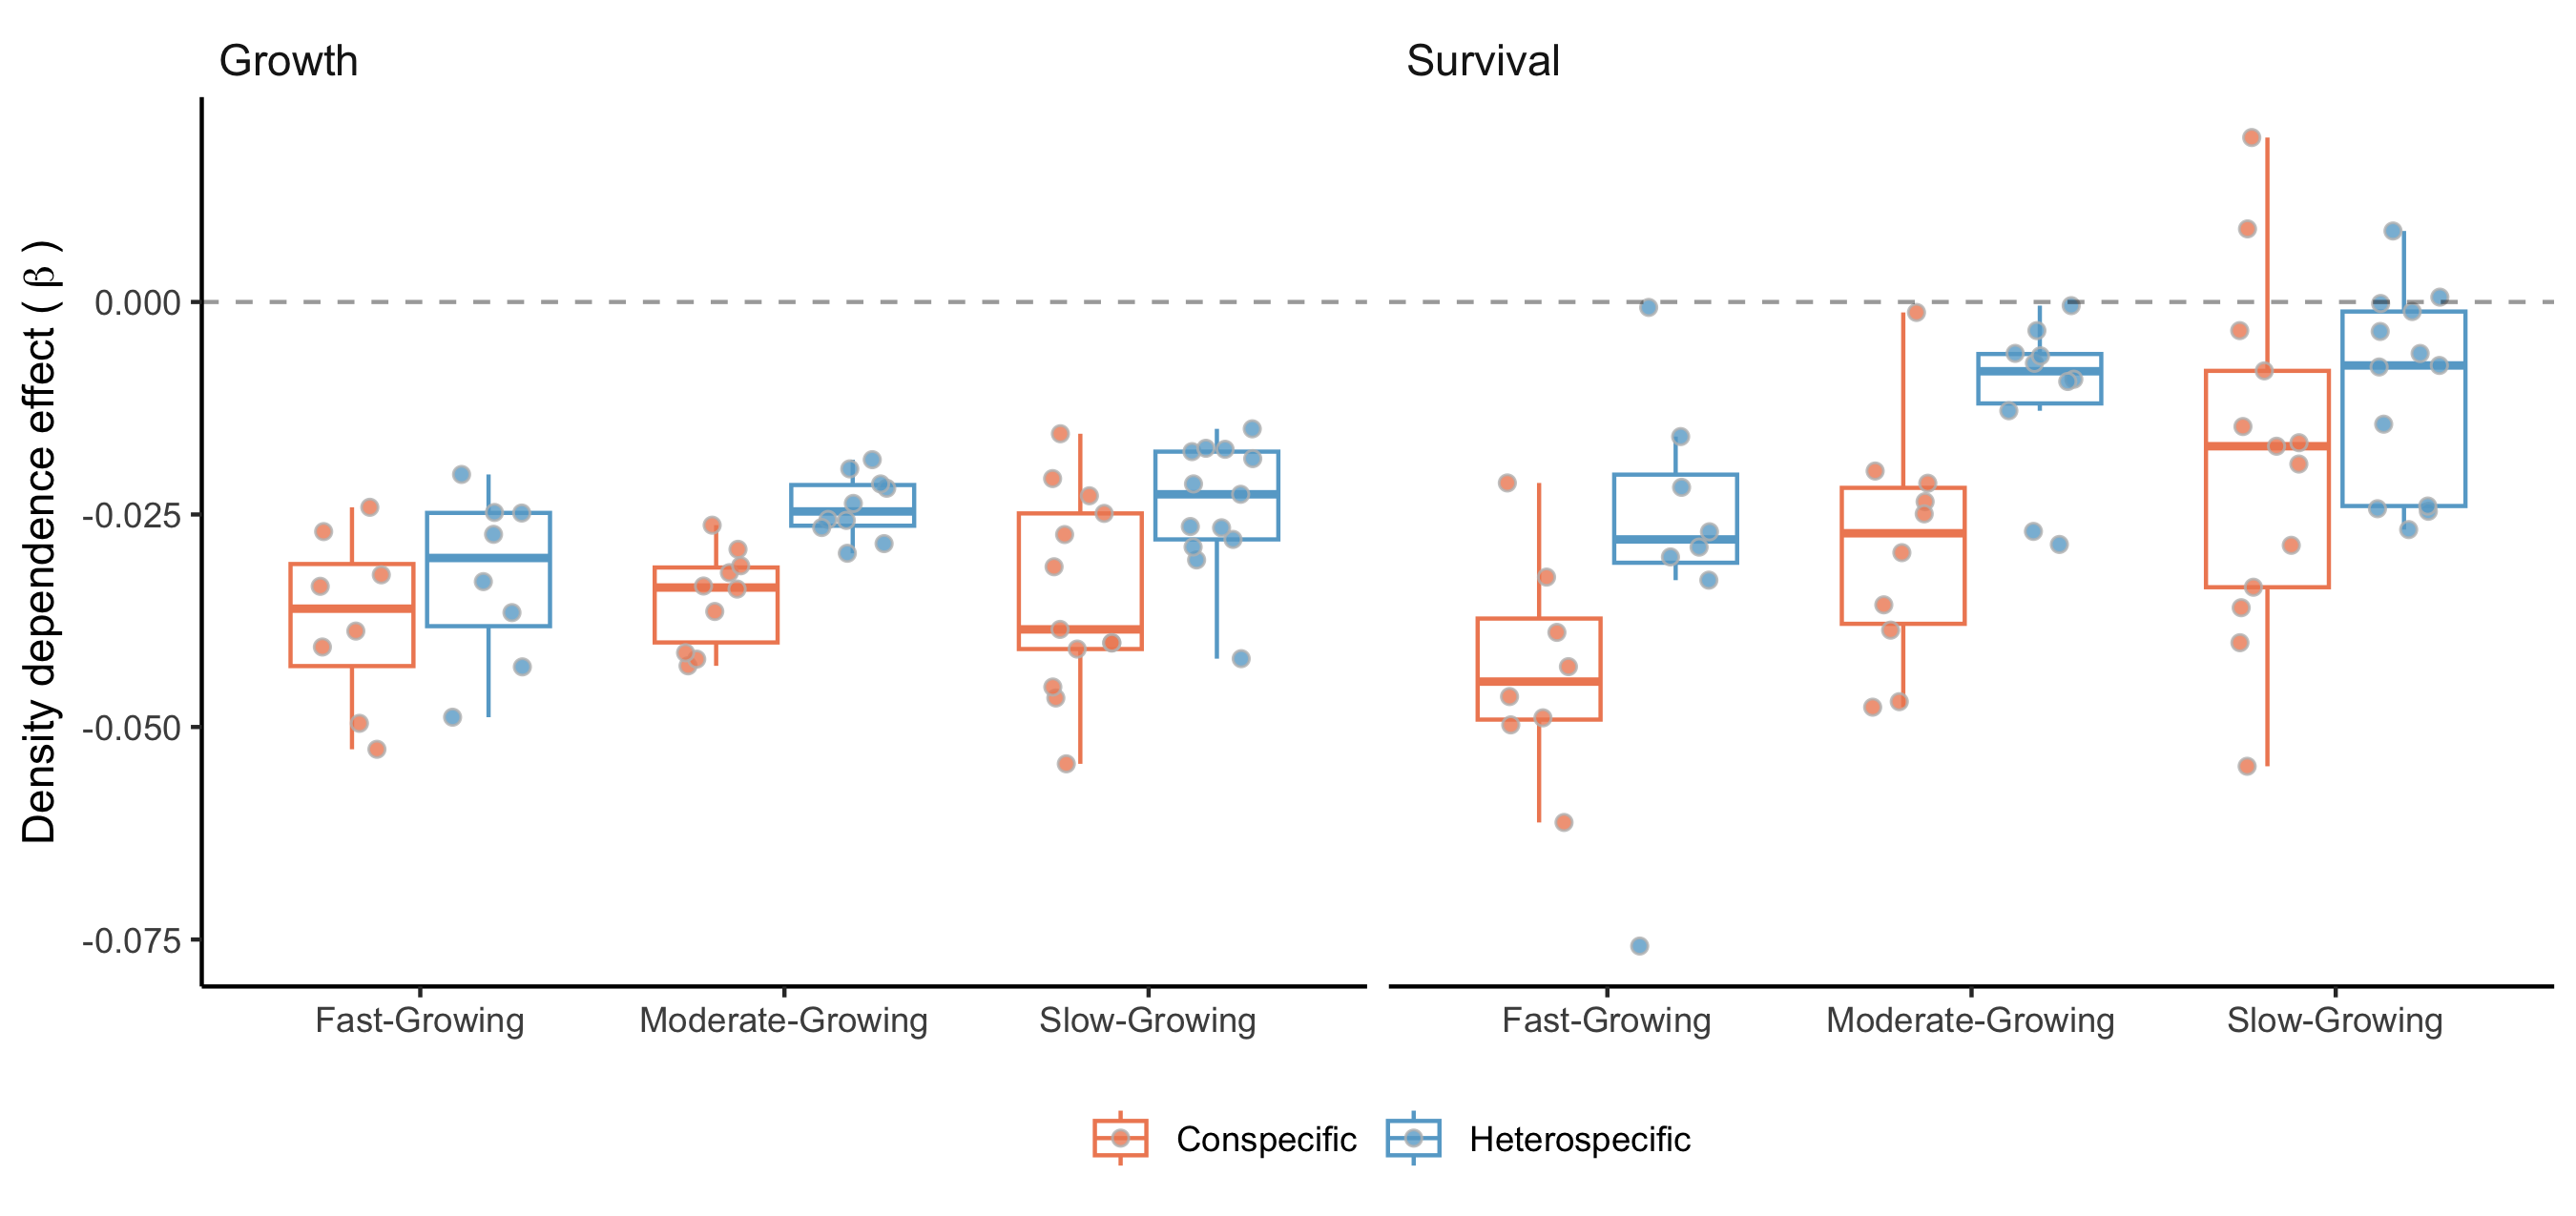
\includegraphics{manuscript/figs/comp_CNDD_vs_growth.png}
\caption[{Posterior distribution for the conspecific (red) and
heterospecific (blue) density dependence for each class of growth rate
\citep{burns1990silvics}.}]{Posterior distribution for the conspecific
(red) and heterospecific (blue) density dependence for each class of
growth rate \citep{burns1990silvics}. The more negative the \(\beta\),
the stronger the competition effect.}
\label{fig:figsupp9_ch2}
\end{figure}
}

\newpage

\hypertarget{fig:figsupp10_ch2}{%
\begin{figure}
\centering
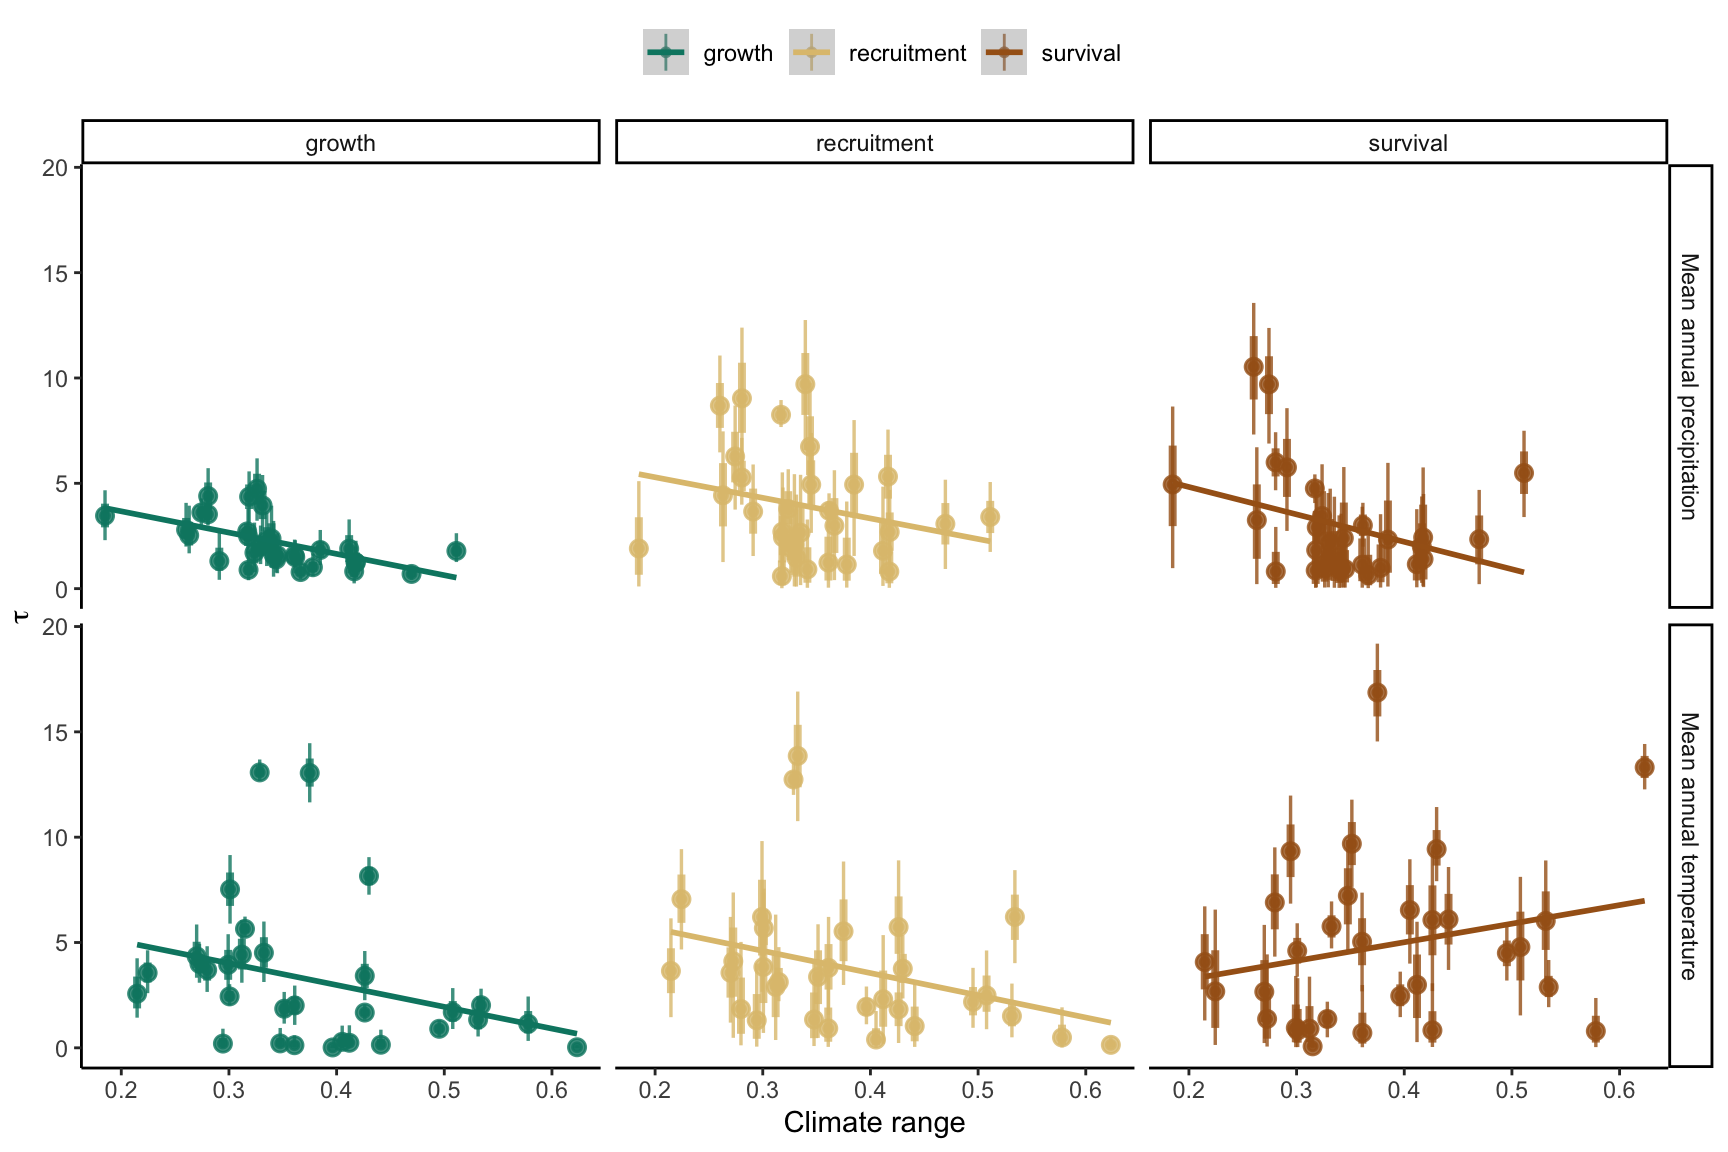
\includegraphics{manuscript/figs/fig-climRangeVsTau-1.png}
\caption[{Climate breadth in function of climate range size.}]{Climate
breadth in function of climate range size. The higher the climate range
size, the more climate conditions the species experienced.}
\label{fig:figsupp10_ch2}
\end{figure}
}

\newpage

\hypertarget{fig:figsupp11_ch2}{%
\begin{figure}
\centering
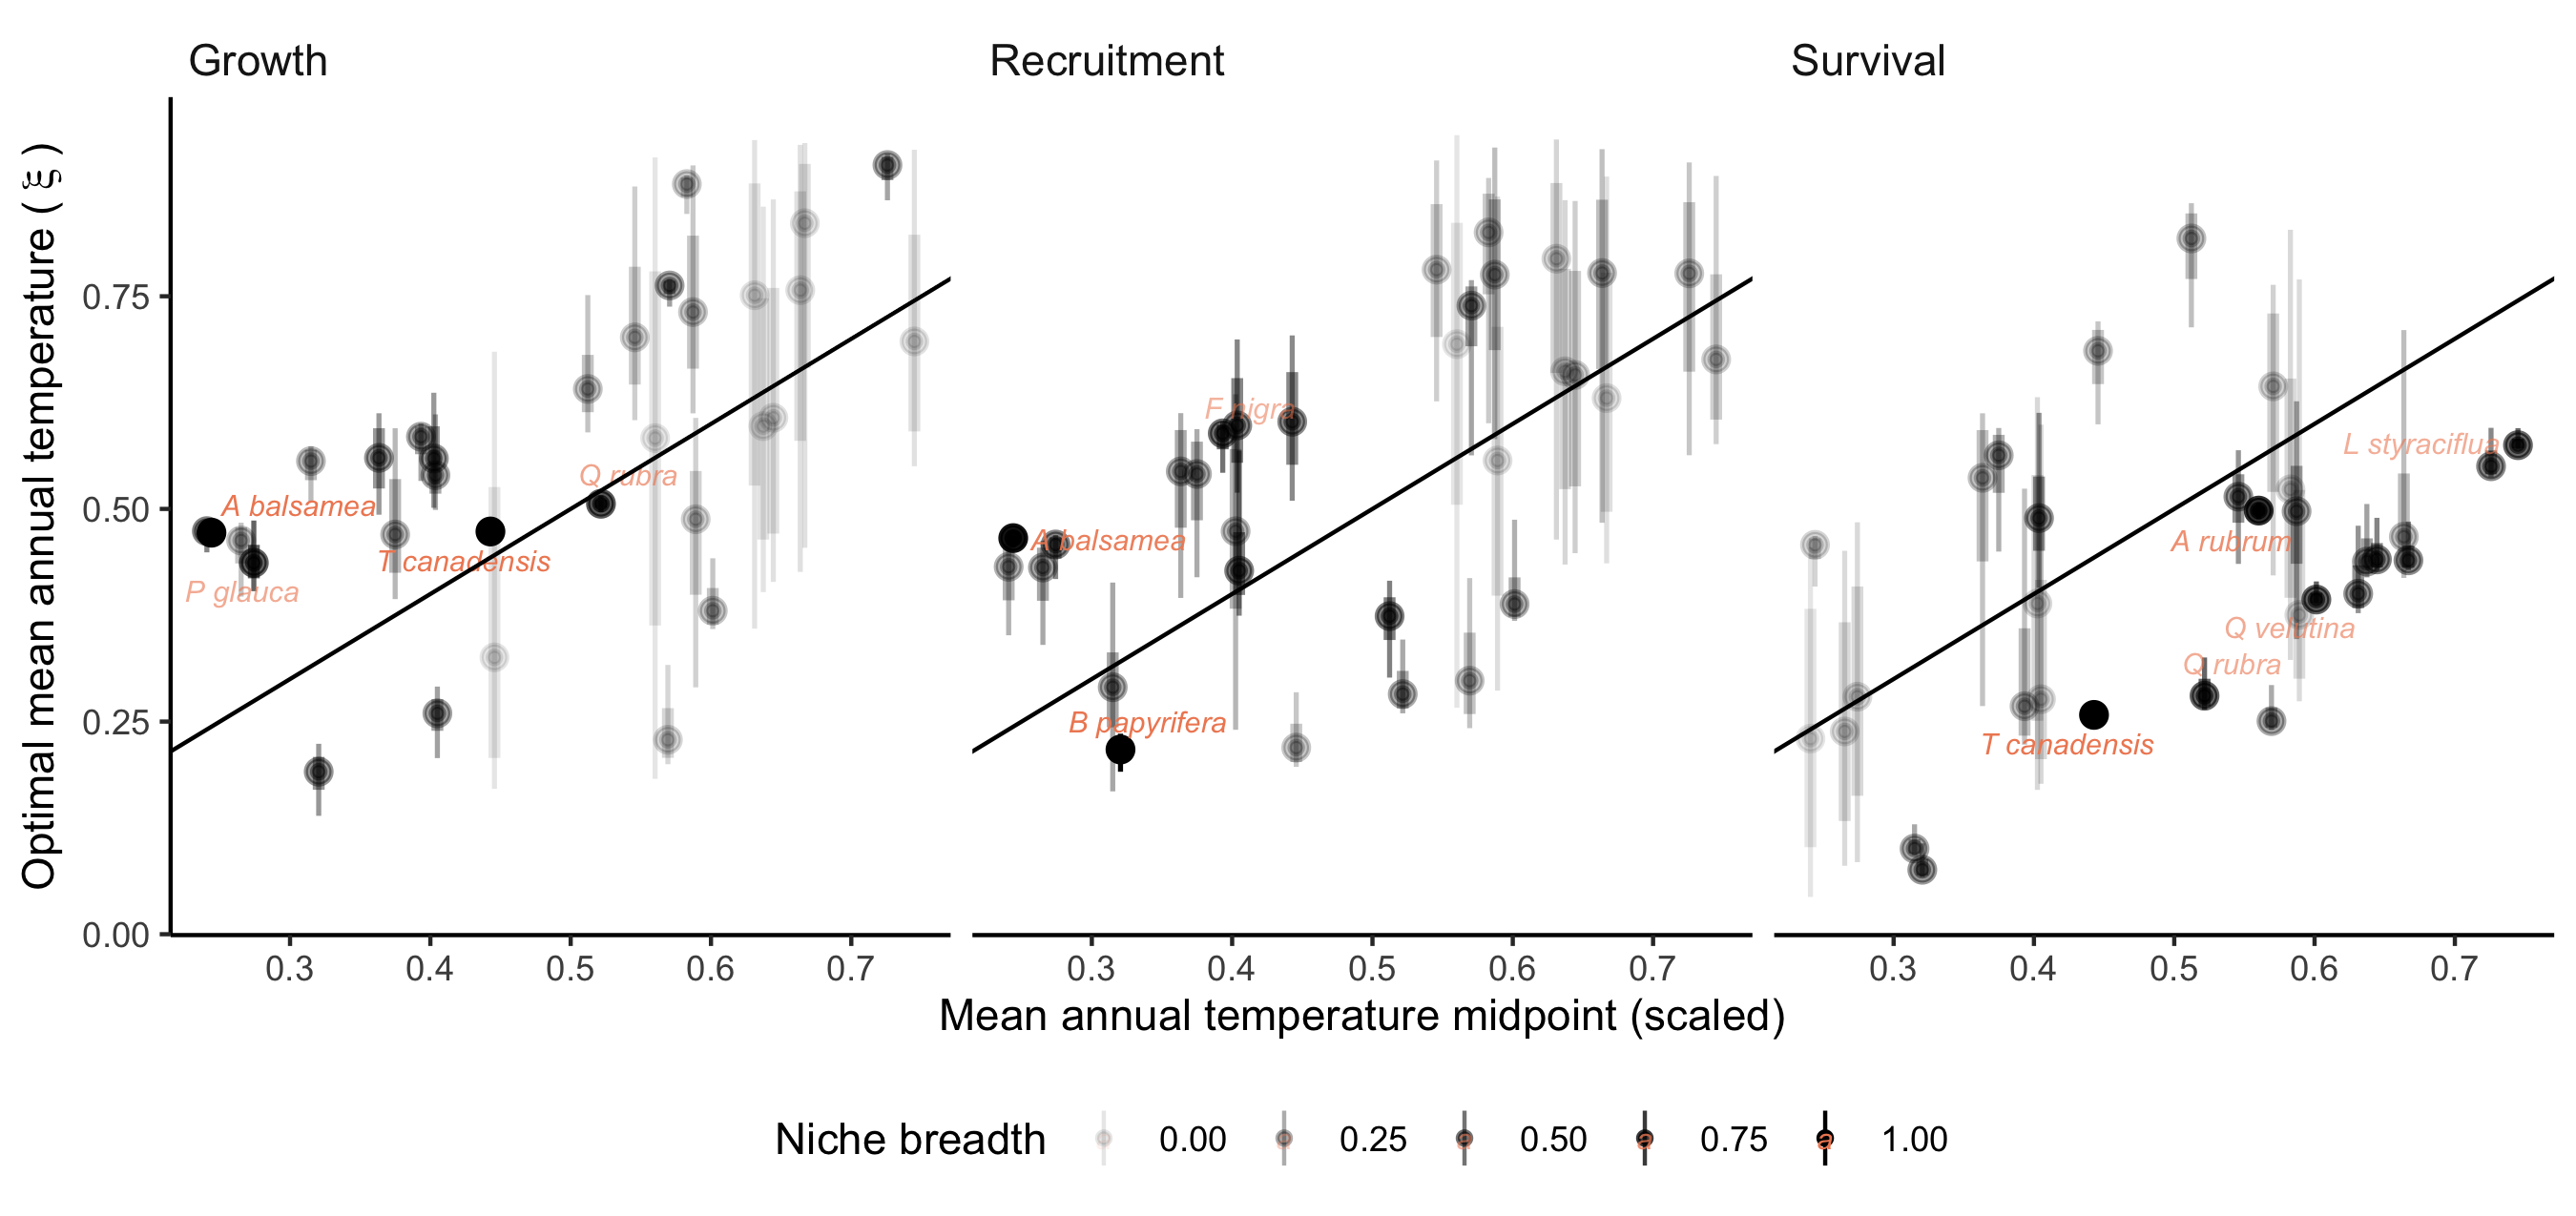
\includegraphics{manuscript/figs/temp_optimal_rangeLocation.png}
\caption[{Correlation between posterior distribution of optimal
temperature (\(\xi_{MAT}\)) and the species' midpoint location across
the mean annual temperature range.}]{Correlation between posterior
distribution of optimal temperature (\(\xi_{MAT}\)) and the species'
midpoint location across the mean annual temperature range. The
transparency of each species point is scaled to be a function of niche
breadth. The closer this value is to zero, the higher the breadth around
the mean. In other words, when climate breadth is zero, the bell-shaped
unimodal function becomes an almost flat line. Colored species names are
those with niche breadth higher than 0.5.}
\label{fig:figsupp11_ch2}
\end{figure}
}

\newpage

\hypertarget{supplementary-mateiral-3}{%
\section{Supplementary Mateiral 3}\label{supplementary-mateiral-3}}

\hypertarget{sensitivity-analysis}{%
\subsection{Sensitivity analysis}\label{sensitivity-analysis}}

Here, we conducted a global sensitivity analysis (GSA) of the population
growth rate (\(\lambda\)) with respect to demographic models.
Sensitivity analysis uses various methods to decompose the total
variance of an outcome into contributions from parameters or input
variables. In structured population models, sensitivity analyses involve
computing partial derivatives of \(\lambda\) to individual parameters,
following \citet{Caswell1978} as:\\

\begin{equation}
 \frac{\partial \lambda}{\partial \theta_i}
\label{eq:sens}\end{equation}\\

where theta represents a vector of \(i\) parameters. However, most
methods quantify the local sensitivity of each parameter separately
while holding all others constant \citep{Saltelli2019}. This approach
can overlook the obscure parameter interactions often common in complex
models. Furthermore, because of the high dimensionality of IPM due to
the large number of parameters, these methods can quickly become
computationally expensive.\\

To address this, we leveraged the efficiency of non-parametric models,
such as random forests, for variable importance classification
\citep{antoniadis2021}. This approach offers speed and suits our study
as it allows us to quantify both sources of variability in \(\lambda\).
It accounts for the sensitivity of \(\lambda\) to each parameter and
considers the uncertainty associated with the parameters. Therefore, a
specific parameter may have higher importance because either \(\lambda\)
is more sensitive to it or because the parameter is more uncertain.\\

We quantified the variability in population growth rate in function of
the parameters using an \emph{insileco} experimental approach.
Specifically, we quantified the variability \(\lambda\) for different
climate conditions, ranging from cold to the center and up to the hot
mean annual temperatures experienced by each species. Furthermore, we
combined the climate conditions with a low and high competition
intensity. We defined the temperature ranges for each species using the
1st, 50th, and 99th percentiles. The low competition was defined as a
population size of \(N = 0.1\), while high competition was set at the
99th percentile of the plot basal area. Precipitation was kept at
optimal conditions computed based on the average optimal precipitation
parameters among growth, survival, and recruitment models.\\

For each species, climate, and competition conditions, we computed
\(\lambda\) 500 times using different draws from the posterior
distribution, setting the plot random effects to zero. The code used for
this analysis can be found in the
\href{https://github.com/willvieira/forest-IPM/tree/master/simulations/sensAnalysis_v3}{\texttt{forest-IPM}}
GitHub repository.\\

\hypertarget{simulation-summary}{%
\subsection{Simulation Summary}\label{simulation-summary}}

The final simulation involved a total of 500 draws across species and
different conditions. The Figure \ref{fig:lambdaDist} illustrates the
distribution of \(\lambda\) computed using 500 random draws from the
posterior distribution of parameters across different climate and
competition conditions.\\

\hypertarget{fig:lambdaDist}{%
\begin{figure}
\centering
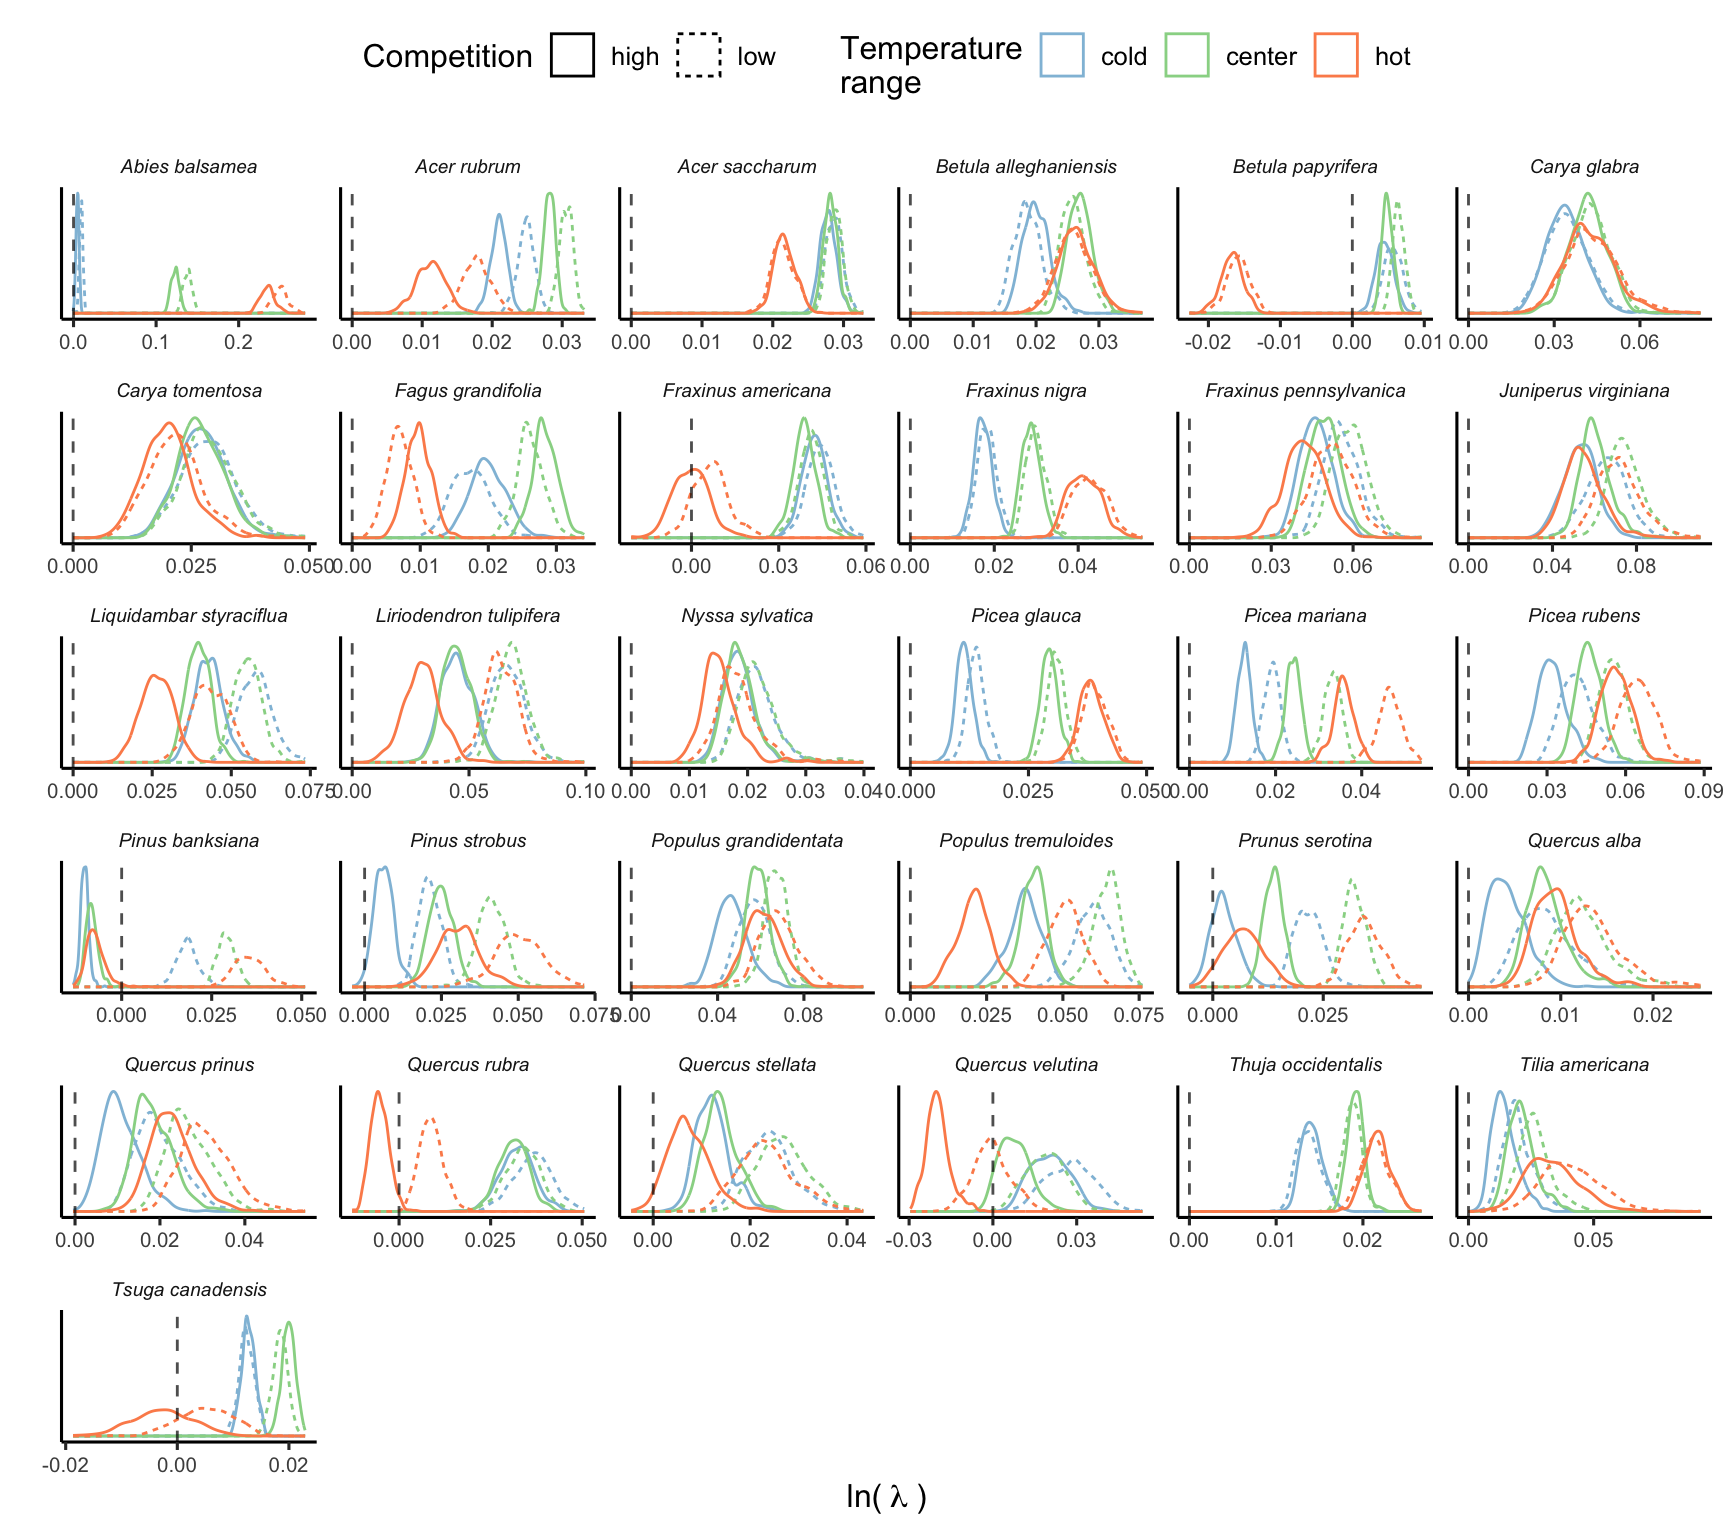
\includegraphics{manuscript/figs/fig-lambdaDist-1.png}
\caption[{Distribution of 500 draws of population growth rate
(\(\lambda\)) for different climate and competition
conditions}]{Distribution of 500 draws of population growth rate
(\(\lambda\)) for different climate and competition conditions}
\label{fig:lambdaDist}
\end{figure}
}

\hypertarget{importance-of-demographic-models}{%
\subsection{Importance of demographic
models}\label{importance-of-demographic-models}}

Random forest is a non-parametric classification or regression model
that ranks each input variable's importance in explaining the variance
of the response variable. We used the permutation method for ranking
variable importance \citep{breiman2001}. This method measures the change
in model performance by individually shuffling (permuting) the values of
each input variable. The greater the change in predictive accuracy with
shuffling input values, the more important the specific variable will
become. This is computed individually for each tree and then averaged
across all \(n\) random trees. Finally, we normalized the importance
output of each regression model so that they sum to 1. We used the R
package \texttt{ranger} with default hyperparameters for fitting the
random forest models \citep{Wright2017}.\\

Figure \ref{fig:rfr2} shows the distribution of \(R^2\) from 20 random
forest replications across different climate and competition conditions.
These values range from 0.2 to 0.9, with an average value of 0.63 across
species and conditions. This variation possibly reflects the uncertainty
in the parameters across species.\\

\hypertarget{fig:rfr2}{%
\begin{figure}
\centering
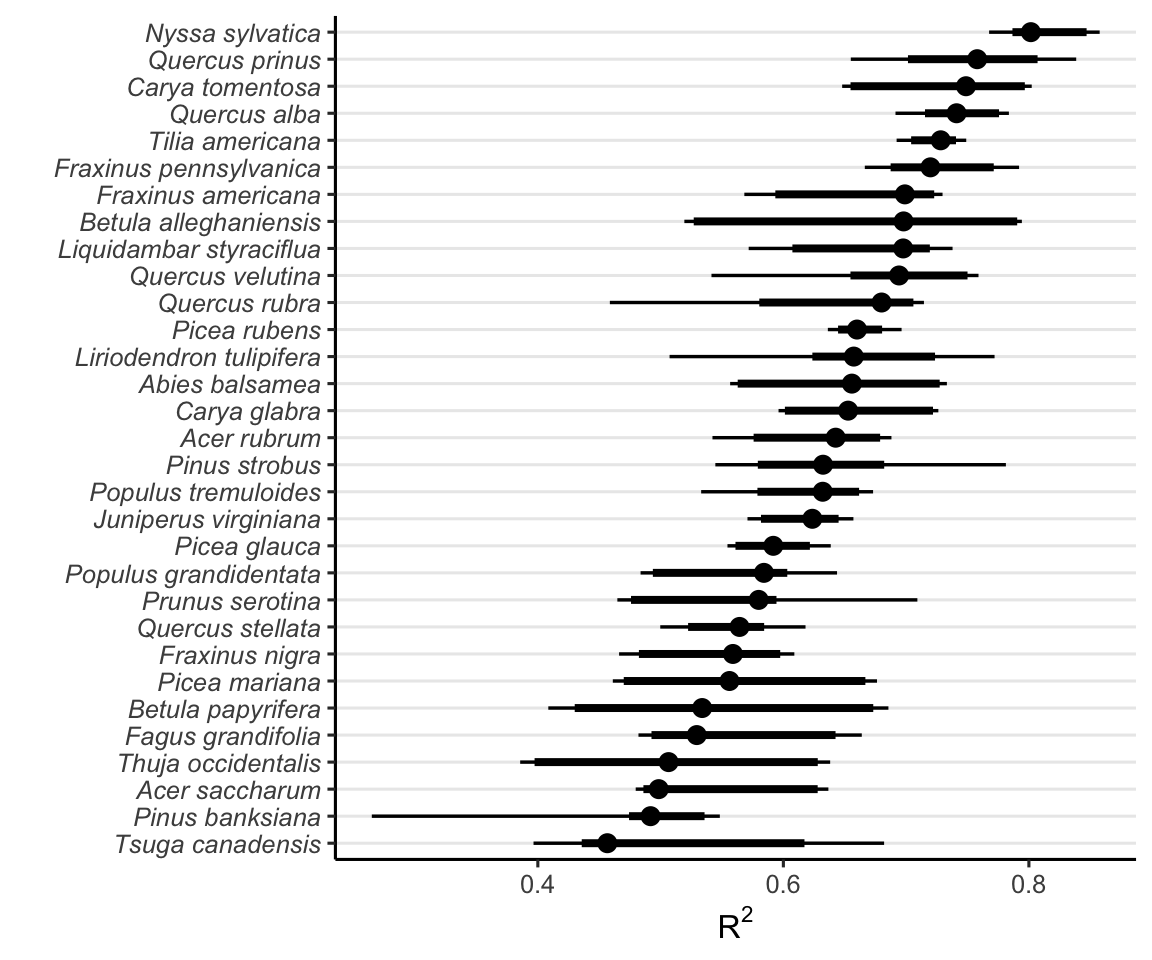
\includegraphics{manuscript/figs/fig-rfr2-1.png}
\caption[{Distribution of \(R^2\) from 20 random forest replications
across different climate and competition conditions.}]{Distribution of
\(R^2\) from 20 random forest replications across different climate and
competition conditions.}
\label{fig:rfr2}
\end{figure}
}

As our primary interest lies in demographic levels rather than parameter
levels, we focus on the combined importance of all parameters for each
demographic model. This splits the total importance among the four
demographic functions of the IPM: growth, survival, recruitment, and
recruited size models. The recruited size model had an insignificant
contribution to \(\lambda\), with nearly all random forest models
showing a contribution below 1\%. Thus, we omitted this model and
concentrated on the growth, survival, and recruitment models, which
collectively explain over 99\% of the variation in \(\lambda\) (Figure
\ref{fig:ternaryLambda}).\\

\hypertarget{fig:ternaryLambda}{%
\begin{figure}
\centering
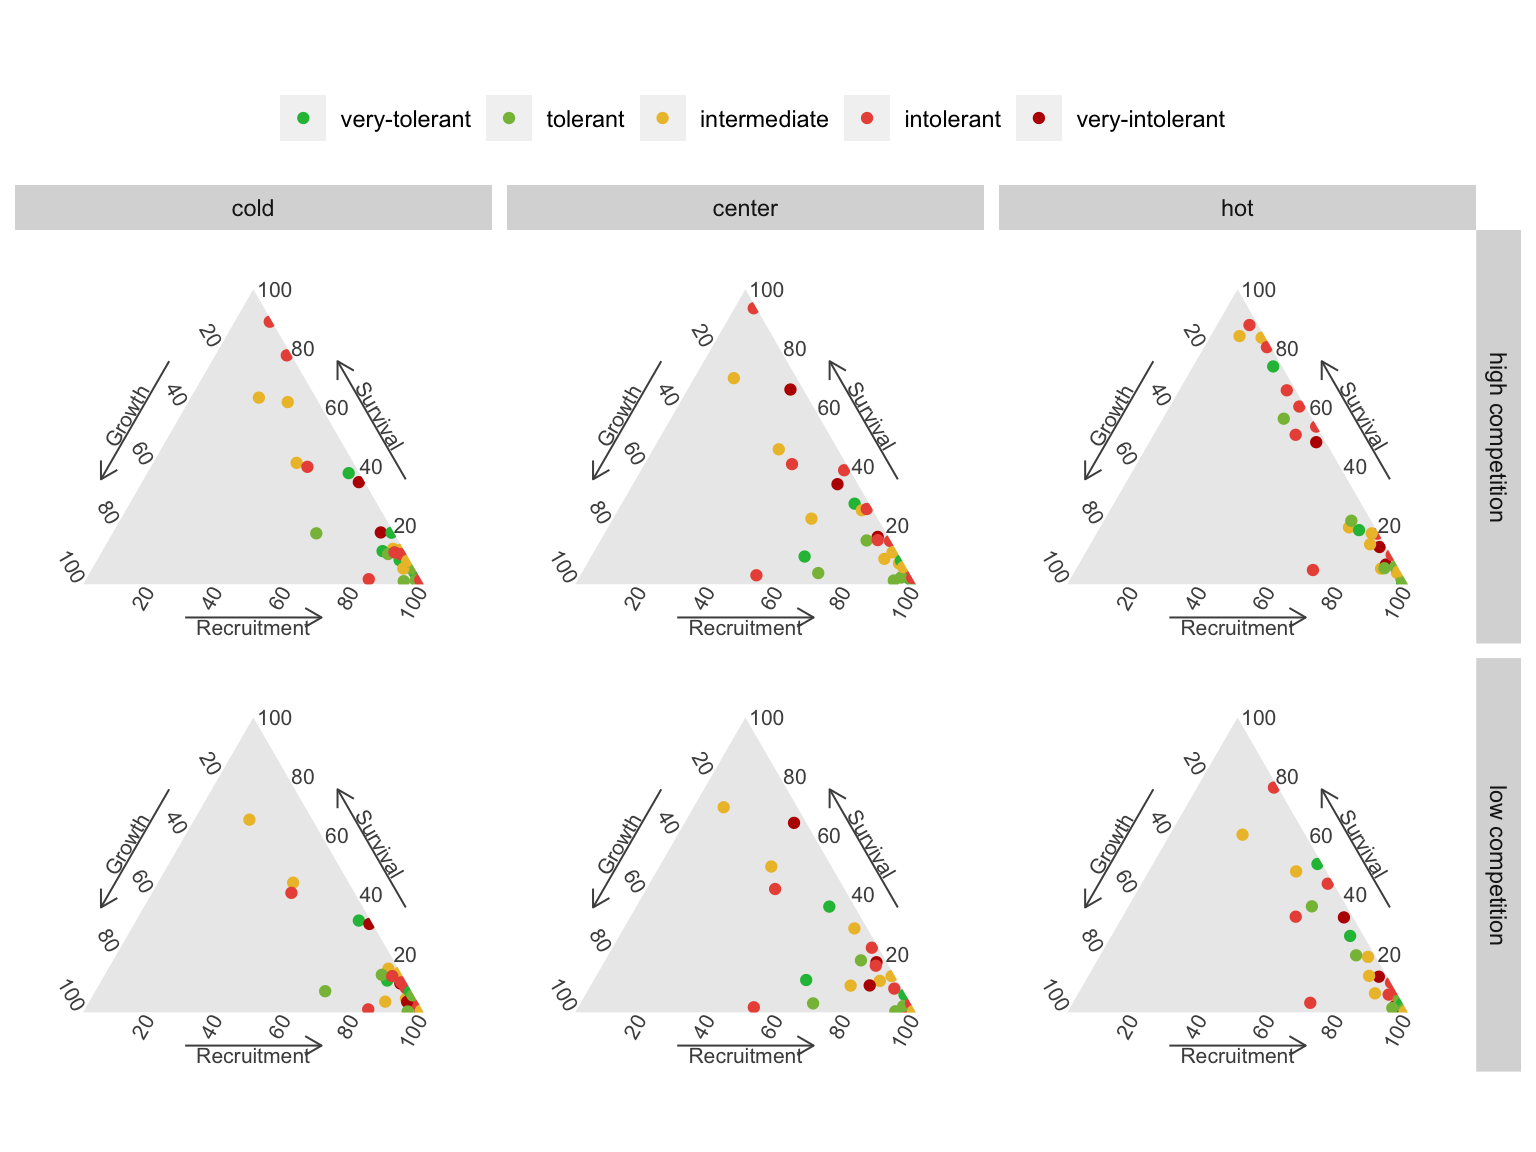
\includegraphics{manuscript/figs/fig-ternaryLambda-1.png}
\caption[{Ternary plot describing the importance distribution among the
growth, survival, and recruitment models.}]{Ternary plot describing the
importance distribution among the growth, survival, and recruitment
models. Color represents the level of shade tolerance
\citep{burns1990silvics}.}
\label{fig:ternaryLambda}
\end{figure}
}

The ternary plots above show the raw importance data from the random
forest, which can be challenging to interpret. The key message is that
variance in \(\lambda\) is primarily explained by the recruitment and
survival demographic models. Furthermore, certain conditions appear to
shift the importance from recruitment to the survival model. In Figure
\ref{fig:recVsMort}, we explore the correlation between the importance
of recruitment and survival under different covariate conditions.\\

\hypertarget{fig:recVsMort}{%
\begin{figure}
\centering
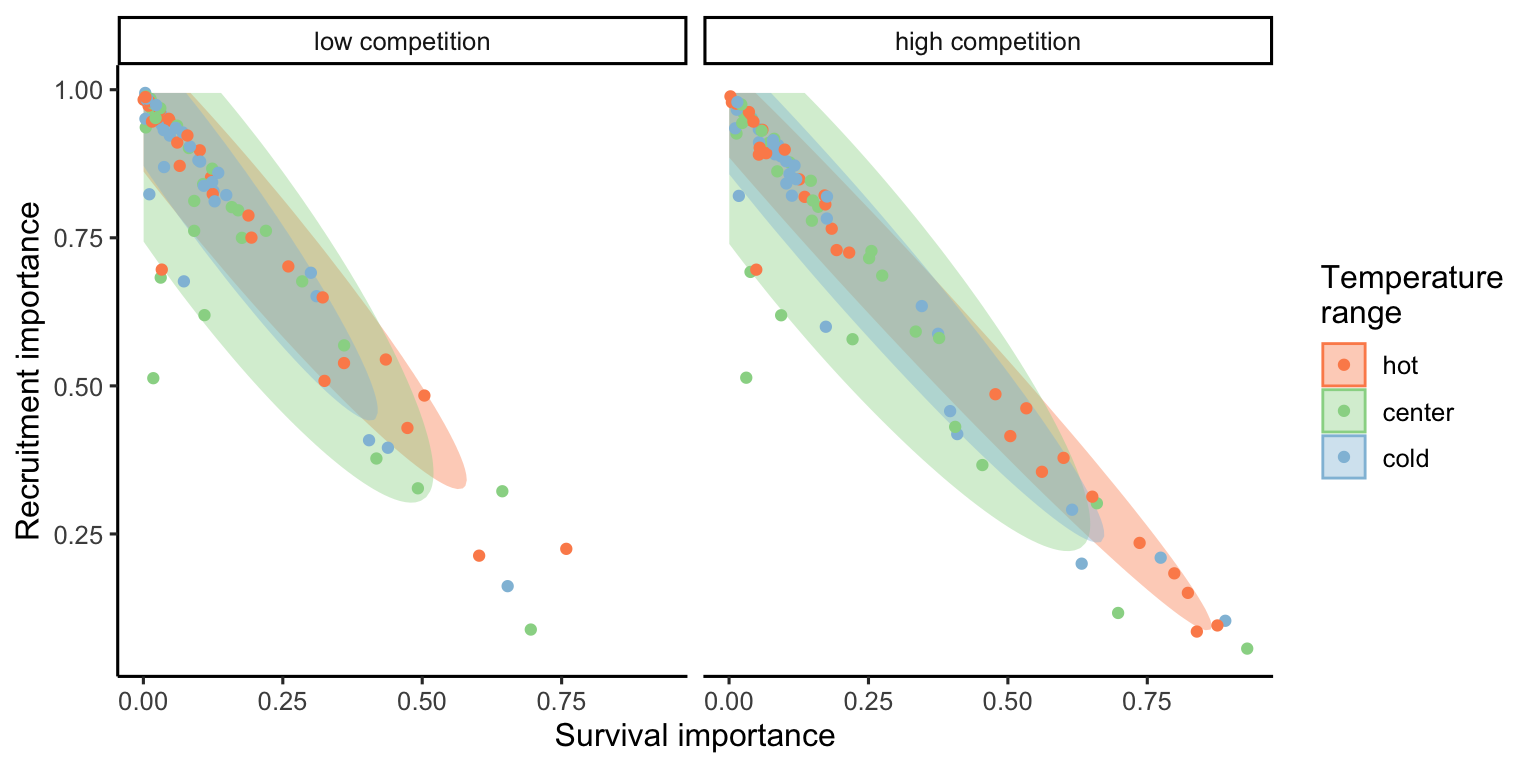
\includegraphics{manuscript/figs/fig-recVsMort-1.png}
\caption[{Correlation between the survival and recruitment relative
importance across the 31 species, climate and competition
conditions.}]{Correlation between the survival and recruitment relative
importance across the 31 species, climate and competition conditions.
Species points are grouped by a Multivariate Normal Density function
with a probability of 90\%.}
\label{fig:recVsMort}
\end{figure}
}

We observe that at low competition, for most species, variations in
\(\lambda\) are primarily explained by recruitment. This pattern
slightly diminishes as we move from the cold range to the center and up
to the hot temperature range. We can observe an overall shift toward the
survival model at high competition intensity, especially in the hot
temperature range.\\

\hypertarget{importance-of-covariates}{%
\subsection{Importance of covariates}\label{importance-of-covariates}}

Similar to assessing parameter importance, we also used the random
forest approach to evaluate the importance of covariates. For
simplicity, we used the same output of the simulations as previously
explained, shifting the explanatory variables from parameters to
covariates.\footnote{This analysis could be expanded to include more
  marginal conditions beyond just cold, center, and hot temperatures and
  low and high competition. However, this would exponentially increase
  the number of simulations.} The Figure \ref{fig:climVsComp} shows the
distribution of relative importance between climate and competition
covariates for each species.\\

\hypertarget{fig:climVsComp}{%
\begin{figure}
\centering
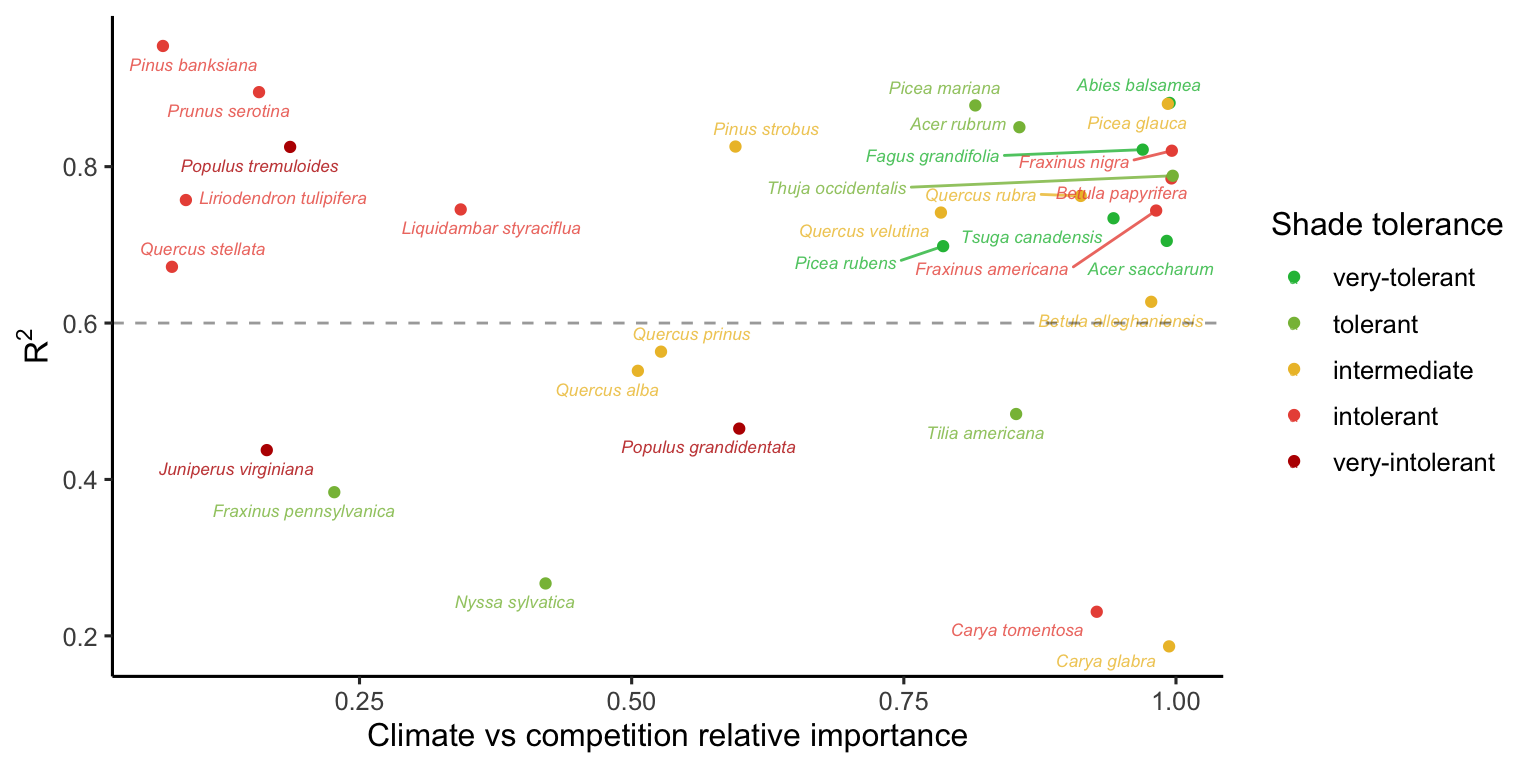
\includegraphics{manuscript/figs/fig-climVsComp-1.png}
\caption[{Distribution of relative importance between climate and
competition covariates according to Random Forest, the respective
\(R^2\).}]{Distribution of relative importance between climate and
competition covariates according to Random Forest, the respective
\(R^2\). The more species are to the right of the panel, the more
climate is important relative to competition. Color represents the level
of shade tolerance \citep{burns1990silvics}}
\label{fig:climVsComp}
\end{figure}
}

\hypertarget{notes-on-conspecific-and-heterospecific-competition-effects}{%
\subsection{Notes on Conspecific and Heterospecific Competition
Effects}\label{notes-on-conspecific-and-heterospecific-competition-effects}}

In the preceding discussion, we did not specify whether we were
considering conspecific or heterospecific competition. For all the
results presented in this chapter, the \emph{high competition} condition
was applied at the heterospecific level, while conspecific competition
was set to a very low proportion. This choice is based on the standard
invasion growth rate metric, or the population growth rate when rare, an
important measure for quantifying population persistence
\citep{lewontin1969}.\\

Additionally, we performed the sensitivity analysis with the same
conditions, except for changing the high competition from heterospecific
to conspecific individuals. We observed that nearly all the variation in
\(\lambda\), previously attributed to the growth model, shifted to the
recruitment model. Also, the importance attributed to the survival model
for certain species at the center and cold temperature conditions
shifted toward the recruitment model. Although we observed this shift,
the overall patterns remained similar to those discussed earlier. The
only exception was the distribution of relative importance between
climate and competition (Figure \ref{fig:climVsComp}), where many
species had an increase in the importance of competition relative to
climate. These observed differences primarily arise from the high
sensitivity of \(\lambda\) to the \(\phi\) parameter.\\

\singlespacing
{\renewcommand{\bibname}{References}
\renewcommand{\bibsection}{\section{\bibname}}
\bibliography{chapter2/manuscript/references}}
\bibliographystyle{styles/myBEAS}
